% main_www.tex -- Citation Equity, The Web Conference 2027 (WWW '27) demo track submission build.
% WORKING DRAFT, 2026-10-24. Owner decisions are marked \owner{...} (blue) and stay visible until he clears them.
%
% Call (https://www2027.thewebconf.org/demos/, re-read 2026-10-24; notes/VENUE.md):
%   - at most 4 pages INCLUDING references, double column, English;
%   - ACM template, recommended \documentclass[sigconf, screen, review]{acmart};
%   - NOT anonymous (single-blind): names and affiliations are listed;
%   - required: a section on the ethical use of data (sec:ethics, "Ethics and use of data");
%   - required: how the demonstration is instantiated at the venue (sec:demo);
%   - external material (code, video, live system) encouraged.
% Build:  bash build.sh         (figures from data, then /opt/homebrew/bin/tectonic --keep-logs main_www.tex)
% Cuts made to fit 4 pages are logged in notes/CUTS.md (cut, never shrink fonts or margins).
% CE = ../citation-equity (the tool repo, read only). Every number in the sections carries a "% src:" comment.
\documentclass[sigconf,screen,review]{acmart}

\usepackage[acm]{smpreprint}% shared interface only (palette, \owner, \figtakeaway, \panel, keys); no layout change
\usepackage{booktabs}
\graphicspath{{figures/}{./}}
% Narrow sigconf columns plus unbreakable numeric citations: allow extra interword stretch instead of overfull lines.
\setlength{\emergencystretch}{2.5em}

% ---- Front matter for the review copy. The conference block is the review default; the camera-ready rights
%      data come from ACM after acceptance.
\setcopyright{none}
\settopmatter{printacmref=false}
% Dates and place from https://www2027.thewebconf.org/ (read 2026-10-24): main conference 12 to 14 May 2027, Dublin, Ireland.
\acmConference[WWW '27]{The ACM Web Conference 2027}{May 12--14, 2027}{Dublin, Ireland}
\acmYear{2027}
\acmISBN{}\acmDOI{}\acmPrice{}% no placeholder ISBN, DOI or price on the review copy

\begin{document}

% Title: the owner picks one of three (notes/OUTLINE.md "Title"); this is the PC critique's suggestion.
\title{Citation Equity: A Writing Tool for AI Search That Tests Its Own Advice}

% Byline: five authors in the owner's order (owner update 2026-10-26). Pegah Zargarian is a Northeastern alumna, so her
% block names the university and country only (no college, no city), as the owner asked.
\author{Mohammad Ali Shehral}
\email{shehral.m@northeastern.edu}
\affiliation{%
  \institution{Northeastern University, Khoury College of Computer Sciences}
  \city{San Jose}
  \state{CA}
  \country{USA}}

\author{Ishan Gupta}
\affiliation{%
  \institution{Northeastern University, Khoury College of Computer Sciences}
  \city{San Jose}
  \state{CA}
  \country{USA}}

\author{Akshay Prajapati}
\email{prajapati.aksh@northeastern.edu}
\affiliation{%
  \institution{Northeastern University, Khoury College of Computer Sciences}
  \city{San Jose}
  \state{CA}
  \country{USA}}

\author{Pegah Zargarian}
\email{zargarian.p@northeastern.edu}
\affiliation{%
  \institution{Northeastern University}
  \country{USA}}

\author{Akram Bayat}
\affiliation{%
  \institution{Northeastern University, Khoury College of Computer Sciences}
  \city{San Jose}
  \state{CA}
  \country{USA}}

\renewcommand{\shortauthors}{Shehral et al.}

% sections/abstract.tex -- Citation Equity, WWW 2027 demo track (draft 2, 2026-10-24; cut to fit 4 pages, notes/CUTS.md)
% Structure per notes/OUTLINE.md "Abstract": context, gap, contribution, rubric outcome, numbers, standard of evidence.
% E1 results exist (CE/experiments/RESULTS_E1.md), so the abstract reports them (notes/OUTLINE.md, notes/NARRATIVE.md "E1").
% Every number carries a % src: comment. CE = ../citation-equity (read only).
\begin{abstract}
AI answer engines now choose which pages a reader sees cited, yet writers get optimization advice with thin evidence, from tools that track brands or rewrite their text.
We present Citation Equity, an open-source writing workspace that runs in the browser.
It shows the graded evidence behind each of its eleven checks, suggests fixes anchored to exact passages that the author applies one at a time, and includes a citation test that separates being retrieved from being cited.
% src (CE c908431): CE/docs/evidence.md line 3 ("scores a draft on eleven checks") and line 34 ("No check is graded strong or moderate today. Nine are mixed and two are untested.")
% src: label text: CE/apps/workspace/components/draft/score-card.tsx line 112 ("A writing checklist, not a forecast.") and CE/README.md
%      line 32 ("so the score is a writing checklist, not a forecast"), CE c908431 (CE/apps/workspace/lib/presets.ts lines 11 to 12
%      keep "not a prediction of citations" in the stance sentence; the paper uses the score card's word everywhere)
Because any null finding counts against a check, none is strongly supported, and the tool calls its score a writing checklist, not a forecast.
% src: scores 40 -> 69 and 42 -> 68 (Standard preset = "foundation" in data/scores.json, four checks unscored, reader's words
%      scored; ce analyze without --questions): data/scores.json (rerun at CE c908431); same figures in CE/samples/README.md
%      line 100 ("foundation score 40 to 69 for espresso, 42 to 68 for RAG")
% src: after_minus_before_exploratory.mean 0.0137, 0.0227, 0.0263, 0.0307 over before 0.164, 0.1784, 0.1538, 0.18 (8% to 17%)
%      in "summary" of CE/experiments/results/sensitivity/sensitivity_{Qwen__Qwen3.5-9B,google__gemma-4-12B-it,Qwen__Qwen3.8-27B,google__gemma-4-31B-it}.json
% src: H2 bar +0.10: CE/experiments/PREREG_sensitivity.md line 30 ("Criteria (fixed before running)", H2); answer_first_minus_before.mean 0.0336, 0.0263, 0.0246, 0.0066, H2 false on all four
On our two sample drafts, following its suggestions raised that score from 40 to 69 and from 42 to 68 but moved mean citation share on four open models by only 1 to 3 points.
% src: E1 (80 queries), E2 (editor Qwen3.8-27B, other judges) and E3 (260 queries pooled): data/e1_results.json;
%      CE/experiments/RESULTS_E1.md, CE/experiments/RESULTS_E2.md, CE/experiments/RESULTS_E3.md; "about 0.03": arm 9 +0.027, arm 12 +0.035, 9W vs original +0.023
Tested one change at a time on real web pages, only adding the reader's own words near the top clearly raised citation, by about 0.03 on a 0-to-1 scale, and kept its sign with another editor and other judges; question headings, cited sources, direct answer first and lists showed no effect larger than 0.03, and attributed quotes were inconclusive.
The tool now scores what helped and marks the rest as unscored notes.
All tests use open models given fixed sources, not live engines.
% src: demo stations: sections/demo.tex (one laptop with Ollama, no venue network for stations 1 and 2)
At the venue, visitors run the loop on an example or their own text on one offline laptop.
\end{abstract}


% CCS concepts (ACM CCS 2012) and keywords.
\begin{CCSXML}
<ccs2012>
<concept><concept_id>10002951.10003260.10003261</concept_id>
<concept_desc>Information systems~Web searching and information discovery</concept_desc>
<concept_significance>500</concept_significance></concept>
<concept><concept_id>10003120.10003121.10003129</concept_id>
<concept_desc>Human-centered computing~Interactive systems and tools</concept_desc>
<concept_significance>300</concept_significance></concept>
</ccs2012>
\end{CCSXML}
\ccsdesc[500]{Information systems~Web searching and information discovery}
\ccsdesc[300]{Human-centered computing~Interactive systems and tools}
\keywords{generative engine optimization, answer engines, citation, writing tools, evidence grading, null results}

% ---- Figure 1: the schematic plus the headline, as the page-1 teaser (sigconf cannot float a figure* onto page 1).
% src (caption): checklist score 40 -> 69 (+29) and 42 -> 68 (+26), Standard ("foundation") preset: data/scores.json
%      (scripts/collect_scores.py, rerun at CE c908431; CE/samples/README.md line 100); citation share +8% to +17% and +0.014 to +0.031:
%      CE/experiments/results/sensitivity/sensitivity_*.json summary.after_minus_before_exploratory and
%      summary.mean_target_share.before; off-topic share <= 0.0031 (max, Qwen3.5-9B): same files, summary.mean_target_share.offtopic.
\begin{teaserfigure}
  \centering
  % fig1_overview.tex -- Figure 1 (figure*, 7.0 in): the tool as a schematic (left) and the headline result (right).
%
% Use inside a figure* (main.tex):   \begin{figure*}% fig1_overview.tex -- Figure 1 (figure*, 7.0 in): the tool as a schematic (left) and the headline result (right).
%
% Use inside a figure* (main.tex):   \begin{figure*}% fig1_overview.tex -- Figure 1 (figure*, 7.0 in): the tool as a schematic (left) and the headline result (right).
%
% Use inside a figure* (main.tex):   \begin{figure*}\input{figures/fig1_overview}\caption{...}\label{fig:overview}\end{figure*}
% Needs: smpreprint.sty (any option; colors sm*, \smfigfont), TikZ libraries arrows.meta, positioning, calc,
%        shadows (loaded by smpreprint.sty), graphicx, and \graphicspath containing figures/ (main.tex) or the
%        current directory (figures/fig1_standalone.tex).
% Right part: fig1_headline.pdf, generated from data by scripts/fig_headline.py (never edited by hand). If it is
%        missing the figure shows a marked frame instead, so the paper still builds.
%
% Schematic contents and where each item comes from (CE = ../citation-equity, read only):
%   draft sheet, the flagged heading "Why espresso turns bitter"  src: CE/samples/espresso-bitterness/before.md line 11
%   stage 1, eleven checks, each graded                           src: CE/docs/evidence.md line 3 (eleven checks), CE c908431
%     pip colors in check order (section headings of CE/docs/evidence.md at CE c908431): standalone-paragraphs untested (l.90),
%     question-headings mixed (l.103), lists mixed (l.119), statistics mixed (l.133), tables untested (l.148), expert-quotes
%     mixed (l.162), cited-sources mixed (l.178), direct-answer-lead mixed (l.193), question-coverage mixed (l.208),
%     comparisons mixed (l.225), reader-words mixed (l.241); "No check is graded strong or moderate today" (l.34)
%   "a writing checklist, not a forecast"                         src: CE/apps/workspace/components/draft/score-card.tsx
%                                                                  line 112 and CE/README.md line 32 (CE c908431)
%   stage 3 label "Test the advice"; the bubble "[1] [2]" stands for numbered citations in an answer (illustrative)
%   stage 2, the card: an edit suggestion the engine emits on the espresso before draft (checkId question-headings,
%     kind edit, title 'End this heading with "?", or reword it as a question'; the check is shown as Not scored since E3, CE c908431)
%                                                                  src: `ce analyze CE/samples/espresso-bitterness/before.md --json`
%                                                                  at CE commit c908431 (rechecked; data/scores.json records the
%                                                                  commit). Question headings is now an unscored note (weight 0):
%                                                                  the card still shows how a ready edit works.
%   Apply / Undo, applied only if the anchored text is unchanged, no bulk action
%                                                                  src: CE/README.md line 13; CE/docs/architecture.md line 81
%   stage 3, draft + competitor pages, BM25 top 8, local model, 8 seeded runs per question, retrieved / cited / share
%     against chance                                               src: CE/samples/README.md line 39; CE/docs/architecture.md lines 52 to 55
%   bottom strip, site readiness: 7 items in CE/docs/evidence.md order (section headings at CE c908431), byline untested (l.275),
%     dates mixed (l.287), structured data mixed (l.299), indexing directives strong (l.313), canonical untested (l.326),
%     crawler access strong (l.336), renders without JavaScript moderate (l.370)
%   who gets cited: answers the author pastes, or the optional live check   src: CE/docs/evidence.md line 387; CE/README.md line 15
%   "never changes the score"                                     src: CE/docs/evidence.md line 262
%   lock: drafts stay on your machine                             src: CE/README.md line 68
%
% Draft caption (the caption lives in main.tex; numbers there come from numbers.tex, not typed):
%   \caption{\figtakeaway{Following the tool's suggestions raises its checklist score by 26 to 29 points, but
%   raises citation share on four open models by only 1 to 3 points.} Left: Citation Equity checks a draft against
%   eleven checks, each shown with the grade of its evidence (1); suggests span-anchored fixes that the author applies
%   one at a time (2); and tests the draft against competitor pages on a local model (3). Site readiness and who
%   gets cited are reported apart and never change the score. \panel{a} Checklist score of the two sample drafts
%   before and after the suggestions (foundation preset, \keyring{smBefore} before, \keyring{smAfter} after; the
%   rise is built in, since the suggestions target the checks). \panel{b} Citation share of the target page in the
%   pre-registered harness on four open models (n = 8 questions x 8 seeds, synthetic packs, target always among the
%   8 sources), one line per model with its relative change, faint lines per sample draft; the after-minus-before
%   contrast is exploratory. Dotted: chance (1 of 8 sources); dashed: the off-topic control. Score marks are hollow
%   and citation marks filled, so the two are never read as one quantity.}
%   [src for the caption's numbers: data/scores.json; CE/experiments/results/sensitivity/sensitivity_*.json]
%
\begingroup
\smfigfont\fontsize{5.5}{6.5}\selectfont
\begin{tikzpicture}[x=1cm, y=1cm, line cap=round, line join=round,
  >={Stealth[length=3.2pt, width=3pt]},
  smpanel/.style={fill=smTint, draw=none, rounded corners=3pt},
  smcard/.style={fill=white, draw=smPaperRule, line width=0.5pt, rounded corners=2.5pt},
  smstage/.style={font=\smfigfont\fontseries{sb}\selectfont\fontsize{7.4}{9}\selectfont, text=smInk, anchor=west,
    inner sep=0pt},
  smnum/.style={circle, fill=smAfter, text=white, inner sep=0pt, minimum size=8.6pt,
    font=\smfigfont\bfseries\fontsize{5.8}{6}\selectfont},
  smsoft/.style={text=smInkSoft, inner sep=0pt},
  smink/.style={text=smInk, inner sep=0pt},
  smnote/.style={text=smInkSoft, inner sep=0pt, font=\smfigfont\itshape\fontsize{5.5}{6.4}\selectfont},
  smhead/.style={text=smInk, inner sep=0pt, font=\smfigfont\fontseries{sb}\selectfont\fontsize{6.2}{7}\selectfont},
  smflow/.style={->, draw=smAfter, line width=0.8pt},
  smthin/.style={->, draw=smInkSoft, line width=0.5pt, >={Stealth[length=2.4pt, width=2.4pt]}},
  smpip/.style={rounded corners=0.8pt, draw=none},
  smbox/.style={fill=white, draw=smRule, line width=0.45pt, rounded corners=2pt, inner xsep=3pt, inner ysep=1.8pt,
    text=smInk},
  smchip/.style={rounded corners=2pt, inner xsep=2pt, inner ysep=1.2pt, font=\smfigfont\fontsize{5.3}{6}\selectfont},
]
% ------------------------------------------------------------------------------------------------- helpers
% \smpip{x}{y}{options}: one grade pip (a small rounded square)
\def\smpip#1#2#3{\fill[smpip, #3] (#1-0.075, #2-0.075) rectangle (#1+0.075, #2+0.075);}
% \smdoc{x}{y}{fill}{draw}: a page glyph with a folded corner
\def\smdoc#1#2#3#4{%
  \filldraw[fill=#3, draw=#4, line width=0.45pt, rounded corners=0.3pt]
    (#1-0.085,#2-0.115) -- (#1+0.085,#2-0.115) -- (#1+0.085,#2+0.06) -- (#1+0.03,#2+0.115) -- (#1-0.085,#2+0.115) -- cycle;}

% Geometry (cm): the schematic spans x 0 to 10.3; the headline panel (7.24 cm = 2.85 in) is right-aligned at 17.78
% (= 7.0 in); main row y 1.42 to 4.85; the bottom strip y 0.05 to 1.2; stage headers at y 5.17.
% columns: draft 0.05-1.95 | stage 1: 2.2-4.4 | stage 2: 4.65-7.45 | stage 3: 7.7-10.3

% ================================================================================================= left: schematic
% ---- stage headers
\node[smstage] at (0.05, 5.17) {Your draft};
\node[smnum] (n1) at (2.32, 5.17) {1};
\node[smstage, right=3pt of n1] {Check};
\node[smnum] (n2) at (4.77, 5.17) {2};
\node[smstage, right=3pt of n2] {Suggest, never rewrite};
\node[smnum] (n3) at (7.86, 5.17) {3};
\node[smstage, right=3pt of n3] {Test the advice};

% ---- the draft sheet
\filldraw[fill=smPaper, draw=smPaperRule, line width=0.5pt, rounded corners=2.5pt,
  drop shadow={opacity=0.10, shadow xshift=0.5pt, shadow yshift=-0.7pt}] (0.05,1.42) rectangle (1.95,4.85);
\begin{scope}[line width=1.4pt, smRule!75]
  \draw[smInk!70, line width=2.0pt] (0.22,4.6) -- (1.45,4.6);          % title
  \foreach \y/\l in {4.36/1.76, 4.23/1.68, 4.10/1.78, 3.97/1.20} \draw (0.22,\y) -- (\l,\y);
  \foreach \y/\l in {3.16/1.78, 3.03/1.70, 2.90/1.80, 2.77/1.58, 2.64/1.76, 2.51/1.05} \draw (0.22,\y) -- (\l,\y);
  \foreach \y/\l in {2.02/1.74, 1.89/1.66, 1.76/1.20} \draw (0.22,\y) -- (\l,\y);
\end{scope}
% the flagged heading, anchored: brand-soft fill and the dotted mark underline
\node[anchor=west, inner xsep=1.5pt, inner ysep=1.1pt, fill=smBrandSoft, rounded corners=1pt, text=smInk, align=left,
  font=\smfigfont\fontseries{sb}\selectfont\fontsize{5.6}{6.4}\selectfont] (span) at (0.16,3.55) {Why espresso\\turns bitter};
\draw[smMark, line width=0.75pt, dash pattern=on 0.6pt off 1.1pt]
  ($(span.south west)+(1.5pt,0.5pt)$) -- ($(span.south east)+(-1.5pt,0.5pt)$);
\draw[smInk!55, line width=1.6pt] (0.22,2.3) -- (1.0,2.3);              % a second, plain heading

% ---- lock: nothing leaves the machine
\filldraw[fill=white, draw=smRule, line width=0.45pt, rounded corners=2.5pt] (0.05,0.05) rectangle (1.95,1.2);
\begin{scope}[shift={(0.31,0.6)}]
  \draw[smAfter, line width=0.95pt] (-0.08,0.02) -- (-0.08,0.11) arc[start angle=180, end angle=0, radius=0.08] -- (0.08,0.02);
  \fill[smAfter, rounded corners=0.8pt] (-0.125,-0.16) rectangle (0.125,0.04);
  \fill[white] (0,-0.06) circle (0.026);
\end{scope}
\node[anchor=west, smink, align=left] at (0.52,0.62)
  {{\fontseries{sb}\selectfont Stays on your}\\{\fontseries{sb}\selectfont machine:} static\\site, no server};

% ---- flow arrows between the stages
\draw[smflow] (1.98,3.8) -- (2.18,3.8);
\draw[smflow] (4.42,3.8) -- (4.63,3.8);
\draw[smflow] (7.47,3.8) -- (7.68,3.8);

% ---- stage 1: check
\fill[smpanel] (2.2,1.42) rectangle (4.4,4.85);
\begin{scope}[shift={(3.3,3.86)}]
  \draw[white, line width=3.4pt] (180:0.58) arc[start angle=180, end angle=0, radius=0.58];
  \draw[smAfter, line width=3.4pt] (180:0.58) arc[start angle=180, end angle=55, radius=0.58];
  \node[smhead] at (0,0.16) {score};
  \node[smsoft, font=\smfigfont\fontsize{5.1}{6}\selectfont] at (0,-0.03) {0 to 100};
\end{scope}
% label matches the score card of the tool at CE c908431 (CE/apps/workspace/components/draft/score-card.tsx line 112,
% "A writing checklist, not a forecast."), as Figure 2 and Section 2.1 say
\node[smnote, align=center] at (3.3,3.42) {a writing checklist,\\ not a forecast};
\node[smink, align=center] at (3.3,2.86) {eleven checks, each shown\\ with its evidence grade};
% pips in check order (grades: CE/docs/evidence.md, see the header); eleven pips centred on the panel (x 3.3)
\foreach \i/\g in {0/smUntested, 1/smMixed, 2/smMixed, 3/smMixed, 4/smUntested, 5/smMixed, 6/smMixed,
                   7/smMixed, 8/smMixed, 9/smMixed, 10/smMixed} {\smpip{2.425+0.175*\i}{2.43}{fill=\g}}
\smpip{2.5}{2.07}{fill=smMixed}    \node[smsoft, anchor=west] at (2.61,2.07) {mixed};
\smpip{3.3}{2.07}{fill=smUntested} \node[smsoft, anchor=west] at (3.41,2.07) {untested};
\node[smnote] at (3.3,1.68) {none strong or moderate};

% ---- stage 2: suggest, never rewrite
\fill[smpanel] (4.65,1.42) rectangle (7.45,4.85);
\filldraw[smcard] (4.78,2.47) rectangle (7.32,4.72);
\node[smchip, fill=smTint, text=smInkSoft, anchor=west] (chk) at (4.86,4.5) {question headings};
\node[smchip, fill=smTint, text=smInkSoft, right=2pt of chk] {not scored};
\node[anchor=north west, smhead] at (4.88,4.27) {End this heading with ``?''};
\node[anchor=west, smsoft, font=\smfigfont\bfseries\fontsize{6}{6}\selectfont, text=smBefore] at (4.88,3.84) {\textminus};
\node[anchor=west, text=smBefore!80!black, inner sep=0pt] at (5.05,3.84) {Why espresso turns bitter};
\node[anchor=west, smsoft, font=\smfigfont\bfseries\fontsize{6}{6}\selectfont, text=smAfter] at (4.88,3.56) {+};
\node[anchor=west, text=smAfter, inner sep=0pt] at (5.05,3.56)
  {Why espresso turns bitter\setlength{\fboxsep}{0.6pt}\colorbox{smBrandSoft}{\fontseries{b}\selectfont ?}};
\node[smnote, anchor=west] at (4.88,3.25) {anchored to the exact words};
\node[smchip, fill=smAfter, text=white, anchor=west, font=\smfigfont\fontseries{sb}\selectfont\fontsize{5.8}{6.5}\selectfont,
  inner xsep=4pt, inner ysep=2pt] (apply) at (4.88,2.9) {Apply};
\node[anchor=west, smsoft, right=6pt of apply] (undo) {Undo};
\node[anchor=west, smsoft, right=6pt of undo] {Skip};
\node[anchor=west, text=smOfftopic, inner sep=0pt] (all) at (4.9,2.13) {Apply all};
\draw[smInkSoft, line width=0.6pt] ($(all.west)+(-1pt,0)$) -- ($(all.east)+(1pt,0)$);
\node[anchor=west, smsoft, right=5pt of all] {no bulk action};
\node[smnote, align=center] at (6.05,1.7) {applies only while the anchored\\ text is unchanged};

% ---- stage 3: test the advice
\fill[smpanel] (7.7,1.42) rectangle (10.3,4.85);
\smdoc{8.17}{4.55}{smAfter}{smAfter}
\foreach \i in {1,...,7} {\smdoc{8.17+0.235*\i}{4.55}{white}{smBefore}}
\node[smsoft, anchor=north] (pages) at (9.0,4.37) {your draft + competitor pages};
\node[smbox, below=7pt of pages] (bm) {BM25 retrieval, top 8};
\node[smbox, below=6pt of bm] (lm) {open model, run locally};
\node[smink, below=6pt of lm] (runs) {8 seeded runs per question};
\draw[smthin] (pages.south) -- (bm.north);
\draw[smthin] (bm.south) -- (lm.north);
\draw[smthin] (lm.south) -- (runs.north);
\foreach \k/\t in {0/{retrieved?}, 1/{cited?}, 2/{share against chance}} {
  \fill[smAfter] (8.33,{2.46-0.24*\k}) circle (0.038);
  \node[anchor=west, smink] at (8.43,{2.46-0.24*\k}) {\t};
}
\node[smnote] at (9.0,1.66) {before vs.\ after, paired test};

% ---- bottom strip: beyond the draft
\draw[smRule, line width=0.5pt, dash pattern=on 2pt off 1.5pt, rounded corners=3pt] (2.2,0.05) rectangle (10.3,1.2);
\node[fill=white, inner xsep=3pt, inner ysep=1pt, anchor=west, text=smInkSoft,
  font=\smfigfont\fontseries{sb}\selectfont\fontsize{5.8}{7}\selectfont] at (2.32,1.2)
  {Beyond the draft: reported apart, never changes the score};
% site readiness
\node[anchor=west, smhead] (sr) at (2.36,0.86) {Site readiness};
\node[smsoft, anchor=west, right=4pt of sr] {can engines reach the page?};
\foreach \i/\g in {0/smUntested, 1/smMixed, 2/smMixed, 3/smStrong, 4/smUntested, 5/smStrong, 6/smModerate}
  {\smpip{2.44+0.194*\i}{0.53}{fill=\g}}
\node[anchor=west, inner sep=0pt, text=smStrong] at (3.86,0.53)
  {\fontseries{sb}\selectfont strong:\fontseries{m}\selectfont\ crawler access, indexing};
\node[smnote, anchor=west] at (2.36,0.25) {seven items, graded on operator documentation};
% who gets cited
\draw[smRule, line width=0.4pt] (6.6,0.18) -- (6.6,1.0);
\node[anchor=west, smhead] at (6.75,0.86) {Who gets cited};
\node[smsoft, anchor=west, align=left] at (6.75,0.42) {AI answers you paste in,\\ or an optional live check};
\begin{scope}[shift={(9.75,0.62)}]
  \filldraw[fill=white, draw=smInkSoft, line width=0.45pt, rounded corners=2pt] (-0.34,-0.18) rectangle (0.34,0.18);
  \fill[white] (-0.15,-0.175) -- (-0.05,-0.175) -- (-0.17,-0.3) -- cycle;
  \draw[smInkSoft, line width=0.45pt] (-0.15,-0.18) -- (-0.17,-0.3) -- (-0.05,-0.18);
  \node[font=\smfigfont\fontseries{sb}\selectfont\fontsize{5.4}{6}\selectfont, text=smAfter, inner sep=0pt] at (0,0) {[1] [2]};
\end{scope}

% ================================================================================================= right: headline
\draw[smRule, line width=0.4pt] (10.43,0.08) -- (10.43,5.3);
\node[anchor=north east, inner sep=0pt] at (17.78,5.385) {%
  \IfFileExists{fig1_headline.pdf}{\includegraphics{fig1_headline.pdf}}{%
  \IfFileExists{figures/fig1_headline.pdf}{\includegraphics{figures/fig1_headline.pdf}}{%
    \tikz\node[draw=smOwner, dashed, text=smOwner, minimum width=7.2cm, minimum height=5.38cm, align=center]
      {[PLACEHOLDER: fig1\_headline.pdf missing;\\ run scripts/fig\_headline.py]};}}};
\end{tikzpicture}
\endgroup
\caption{...}\label{fig:overview}\end{figure*}
% Needs: smpreprint.sty (any option; colors sm*, \smfigfont), TikZ libraries arrows.meta, positioning, calc,
%        shadows (loaded by smpreprint.sty), graphicx, and \graphicspath containing figures/ (main.tex) or the
%        current directory (figures/fig1_standalone.tex).
% Right part: fig1_headline.pdf, generated from data by scripts/fig_headline.py (never edited by hand). If it is
%        missing the figure shows a marked frame instead, so the paper still builds.
%
% Schematic contents and where each item comes from (CE = ../citation-equity, read only):
%   draft sheet, the flagged heading "Why espresso turns bitter"  src: CE/samples/espresso-bitterness/before.md line 11
%   stage 1, eleven checks, each graded                           src: CE/docs/evidence.md line 3 (eleven checks), CE c908431
%     pip colors in check order (section headings of CE/docs/evidence.md at CE c908431): standalone-paragraphs untested (l.90),
%     question-headings mixed (l.103), lists mixed (l.119), statistics mixed (l.133), tables untested (l.148), expert-quotes
%     mixed (l.162), cited-sources mixed (l.178), direct-answer-lead mixed (l.193), question-coverage mixed (l.208),
%     comparisons mixed (l.225), reader-words mixed (l.241); "No check is graded strong or moderate today" (l.34)
%   "a writing checklist, not a forecast"                         src: CE/apps/workspace/components/draft/score-card.tsx
%                                                                  line 112 and CE/README.md line 32 (CE c908431)
%   stage 3 label "Test the advice"; the bubble "[1] [2]" stands for numbered citations in an answer (illustrative)
%   stage 2, the card: an edit suggestion the engine emits on the espresso before draft (checkId question-headings,
%     kind edit, title 'End this heading with "?", or reword it as a question'; the check is shown as Not scored since E3, CE c908431)
%                                                                  src: `ce analyze CE/samples/espresso-bitterness/before.md --json`
%                                                                  at CE commit c908431 (rechecked; data/scores.json records the
%                                                                  commit). Question headings is now an unscored note (weight 0):
%                                                                  the card still shows how a ready edit works.
%   Apply / Undo, applied only if the anchored text is unchanged, no bulk action
%                                                                  src: CE/README.md line 13; CE/docs/architecture.md line 81
%   stage 3, draft + competitor pages, BM25 top 8, local model, 8 seeded runs per question, retrieved / cited / share
%     against chance                                               src: CE/samples/README.md line 39; CE/docs/architecture.md lines 52 to 55
%   bottom strip, site readiness: 7 items in CE/docs/evidence.md order (section headings at CE c908431), byline untested (l.275),
%     dates mixed (l.287), structured data mixed (l.299), indexing directives strong (l.313), canonical untested (l.326),
%     crawler access strong (l.336), renders without JavaScript moderate (l.370)
%   who gets cited: answers the author pastes, or the optional live check   src: CE/docs/evidence.md line 387; CE/README.md line 15
%   "never changes the score"                                     src: CE/docs/evidence.md line 262
%   lock: drafts stay on your machine                             src: CE/README.md line 68
%
% Draft caption (the caption lives in main.tex; numbers there come from numbers.tex, not typed):
%   \caption{\figtakeaway{Following the tool's suggestions raises its checklist score by 26 to 29 points, but
%   raises citation share on four open models by only 1 to 3 points.} Left: Citation Equity checks a draft against
%   eleven checks, each shown with the grade of its evidence (1); suggests span-anchored fixes that the author applies
%   one at a time (2); and tests the draft against competitor pages on a local model (3). Site readiness and who
%   gets cited are reported apart and never change the score. \panel{a} Checklist score of the two sample drafts
%   before and after the suggestions (foundation preset, \keyring{smBefore} before, \keyring{smAfter} after; the
%   rise is built in, since the suggestions target the checks). \panel{b} Citation share of the target page in the
%   pre-registered harness on four open models (n = 8 questions x 8 seeds, synthetic packs, target always among the
%   8 sources), one line per model with its relative change, faint lines per sample draft; the after-minus-before
%   contrast is exploratory. Dotted: chance (1 of 8 sources); dashed: the off-topic control. Score marks are hollow
%   and citation marks filled, so the two are never read as one quantity.}
%   [src for the caption's numbers: data/scores.json; CE/experiments/results/sensitivity/sensitivity_*.json]
%
\begingroup
\smfigfont\fontsize{5.5}{6.5}\selectfont
\begin{tikzpicture}[x=1cm, y=1cm, line cap=round, line join=round,
  >={Stealth[length=3.2pt, width=3pt]},
  smpanel/.style={fill=smTint, draw=none, rounded corners=3pt},
  smcard/.style={fill=white, draw=smPaperRule, line width=0.5pt, rounded corners=2.5pt},
  smstage/.style={font=\smfigfont\fontseries{sb}\selectfont\fontsize{7.4}{9}\selectfont, text=smInk, anchor=west,
    inner sep=0pt},
  smnum/.style={circle, fill=smAfter, text=white, inner sep=0pt, minimum size=8.6pt,
    font=\smfigfont\bfseries\fontsize{5.8}{6}\selectfont},
  smsoft/.style={text=smInkSoft, inner sep=0pt},
  smink/.style={text=smInk, inner sep=0pt},
  smnote/.style={text=smInkSoft, inner sep=0pt, font=\smfigfont\itshape\fontsize{5.5}{6.4}\selectfont},
  smhead/.style={text=smInk, inner sep=0pt, font=\smfigfont\fontseries{sb}\selectfont\fontsize{6.2}{7}\selectfont},
  smflow/.style={->, draw=smAfter, line width=0.8pt},
  smthin/.style={->, draw=smInkSoft, line width=0.5pt, >={Stealth[length=2.4pt, width=2.4pt]}},
  smpip/.style={rounded corners=0.8pt, draw=none},
  smbox/.style={fill=white, draw=smRule, line width=0.45pt, rounded corners=2pt, inner xsep=3pt, inner ysep=1.8pt,
    text=smInk},
  smchip/.style={rounded corners=2pt, inner xsep=2pt, inner ysep=1.2pt, font=\smfigfont\fontsize{5.3}{6}\selectfont},
]
% ------------------------------------------------------------------------------------------------- helpers
% \smpip{x}{y}{options}: one grade pip (a small rounded square)
\def\smpip#1#2#3{\fill[smpip, #3] (#1-0.075, #2-0.075) rectangle (#1+0.075, #2+0.075);}
% \smdoc{x}{y}{fill}{draw}: a page glyph with a folded corner
\def\smdoc#1#2#3#4{%
  \filldraw[fill=#3, draw=#4, line width=0.45pt, rounded corners=0.3pt]
    (#1-0.085,#2-0.115) -- (#1+0.085,#2-0.115) -- (#1+0.085,#2+0.06) -- (#1+0.03,#2+0.115) -- (#1-0.085,#2+0.115) -- cycle;}

% Geometry (cm): the schematic spans x 0 to 10.3; the headline panel (7.24 cm = 2.85 in) is right-aligned at 17.78
% (= 7.0 in); main row y 1.42 to 4.85; the bottom strip y 0.05 to 1.2; stage headers at y 5.17.
% columns: draft 0.05-1.95 | stage 1: 2.2-4.4 | stage 2: 4.65-7.45 | stage 3: 7.7-10.3

% ================================================================================================= left: schematic
% ---- stage headers
\node[smstage] at (0.05, 5.17) {Your draft};
\node[smnum] (n1) at (2.32, 5.17) {1};
\node[smstage, right=3pt of n1] {Check};
\node[smnum] (n2) at (4.77, 5.17) {2};
\node[smstage, right=3pt of n2] {Suggest, never rewrite};
\node[smnum] (n3) at (7.86, 5.17) {3};
\node[smstage, right=3pt of n3] {Test the advice};

% ---- the draft sheet
\filldraw[fill=smPaper, draw=smPaperRule, line width=0.5pt, rounded corners=2.5pt,
  drop shadow={opacity=0.10, shadow xshift=0.5pt, shadow yshift=-0.7pt}] (0.05,1.42) rectangle (1.95,4.85);
\begin{scope}[line width=1.4pt, smRule!75]
  \draw[smInk!70, line width=2.0pt] (0.22,4.6) -- (1.45,4.6);          % title
  \foreach \y/\l in {4.36/1.76, 4.23/1.68, 4.10/1.78, 3.97/1.20} \draw (0.22,\y) -- (\l,\y);
  \foreach \y/\l in {3.16/1.78, 3.03/1.70, 2.90/1.80, 2.77/1.58, 2.64/1.76, 2.51/1.05} \draw (0.22,\y) -- (\l,\y);
  \foreach \y/\l in {2.02/1.74, 1.89/1.66, 1.76/1.20} \draw (0.22,\y) -- (\l,\y);
\end{scope}
% the flagged heading, anchored: brand-soft fill and the dotted mark underline
\node[anchor=west, inner xsep=1.5pt, inner ysep=1.1pt, fill=smBrandSoft, rounded corners=1pt, text=smInk, align=left,
  font=\smfigfont\fontseries{sb}\selectfont\fontsize{5.6}{6.4}\selectfont] (span) at (0.16,3.55) {Why espresso\\turns bitter};
\draw[smMark, line width=0.75pt, dash pattern=on 0.6pt off 1.1pt]
  ($(span.south west)+(1.5pt,0.5pt)$) -- ($(span.south east)+(-1.5pt,0.5pt)$);
\draw[smInk!55, line width=1.6pt] (0.22,2.3) -- (1.0,2.3);              % a second, plain heading

% ---- lock: nothing leaves the machine
\filldraw[fill=white, draw=smRule, line width=0.45pt, rounded corners=2.5pt] (0.05,0.05) rectangle (1.95,1.2);
\begin{scope}[shift={(0.31,0.6)}]
  \draw[smAfter, line width=0.95pt] (-0.08,0.02) -- (-0.08,0.11) arc[start angle=180, end angle=0, radius=0.08] -- (0.08,0.02);
  \fill[smAfter, rounded corners=0.8pt] (-0.125,-0.16) rectangle (0.125,0.04);
  \fill[white] (0,-0.06) circle (0.026);
\end{scope}
\node[anchor=west, smink, align=left] at (0.52,0.62)
  {{\fontseries{sb}\selectfont Stays on your}\\{\fontseries{sb}\selectfont machine:} static\\site, no server};

% ---- flow arrows between the stages
\draw[smflow] (1.98,3.8) -- (2.18,3.8);
\draw[smflow] (4.42,3.8) -- (4.63,3.8);
\draw[smflow] (7.47,3.8) -- (7.68,3.8);

% ---- stage 1: check
\fill[smpanel] (2.2,1.42) rectangle (4.4,4.85);
\begin{scope}[shift={(3.3,3.86)}]
  \draw[white, line width=3.4pt] (180:0.58) arc[start angle=180, end angle=0, radius=0.58];
  \draw[smAfter, line width=3.4pt] (180:0.58) arc[start angle=180, end angle=55, radius=0.58];
  \node[smhead] at (0,0.16) {score};
  \node[smsoft, font=\smfigfont\fontsize{5.1}{6}\selectfont] at (0,-0.03) {0 to 100};
\end{scope}
% label matches the score card of the tool at CE c908431 (CE/apps/workspace/components/draft/score-card.tsx line 112,
% "A writing checklist, not a forecast."), as Figure 2 and Section 2.1 say
\node[smnote, align=center] at (3.3,3.42) {a writing checklist,\\ not a forecast};
\node[smink, align=center] at (3.3,2.86) {eleven checks, each shown\\ with its evidence grade};
% pips in check order (grades: CE/docs/evidence.md, see the header); eleven pips centred on the panel (x 3.3)
\foreach \i/\g in {0/smUntested, 1/smMixed, 2/smMixed, 3/smMixed, 4/smUntested, 5/smMixed, 6/smMixed,
                   7/smMixed, 8/smMixed, 9/smMixed, 10/smMixed} {\smpip{2.425+0.175*\i}{2.43}{fill=\g}}
\smpip{2.5}{2.07}{fill=smMixed}    \node[smsoft, anchor=west] at (2.61,2.07) {mixed};
\smpip{3.3}{2.07}{fill=smUntested} \node[smsoft, anchor=west] at (3.41,2.07) {untested};
\node[smnote] at (3.3,1.68) {none strong or moderate};

% ---- stage 2: suggest, never rewrite
\fill[smpanel] (4.65,1.42) rectangle (7.45,4.85);
\filldraw[smcard] (4.78,2.47) rectangle (7.32,4.72);
\node[smchip, fill=smTint, text=smInkSoft, anchor=west] (chk) at (4.86,4.5) {question headings};
\node[smchip, fill=smTint, text=smInkSoft, right=2pt of chk] {not scored};
\node[anchor=north west, smhead] at (4.88,4.27) {End this heading with ``?''};
\node[anchor=west, smsoft, font=\smfigfont\bfseries\fontsize{6}{6}\selectfont, text=smBefore] at (4.88,3.84) {\textminus};
\node[anchor=west, text=smBefore!80!black, inner sep=0pt] at (5.05,3.84) {Why espresso turns bitter};
\node[anchor=west, smsoft, font=\smfigfont\bfseries\fontsize{6}{6}\selectfont, text=smAfter] at (4.88,3.56) {+};
\node[anchor=west, text=smAfter, inner sep=0pt] at (5.05,3.56)
  {Why espresso turns bitter\setlength{\fboxsep}{0.6pt}\colorbox{smBrandSoft}{\fontseries{b}\selectfont ?}};
\node[smnote, anchor=west] at (4.88,3.25) {anchored to the exact words};
\node[smchip, fill=smAfter, text=white, anchor=west, font=\smfigfont\fontseries{sb}\selectfont\fontsize{5.8}{6.5}\selectfont,
  inner xsep=4pt, inner ysep=2pt] (apply) at (4.88,2.9) {Apply};
\node[anchor=west, smsoft, right=6pt of apply] (undo) {Undo};
\node[anchor=west, smsoft, right=6pt of undo] {Skip};
\node[anchor=west, text=smOfftopic, inner sep=0pt] (all) at (4.9,2.13) {Apply all};
\draw[smInkSoft, line width=0.6pt] ($(all.west)+(-1pt,0)$) -- ($(all.east)+(1pt,0)$);
\node[anchor=west, smsoft, right=5pt of all] {no bulk action};
\node[smnote, align=center] at (6.05,1.7) {applies only while the anchored\\ text is unchanged};

% ---- stage 3: test the advice
\fill[smpanel] (7.7,1.42) rectangle (10.3,4.85);
\smdoc{8.17}{4.55}{smAfter}{smAfter}
\foreach \i in {1,...,7} {\smdoc{8.17+0.235*\i}{4.55}{white}{smBefore}}
\node[smsoft, anchor=north] (pages) at (9.0,4.37) {your draft + competitor pages};
\node[smbox, below=7pt of pages] (bm) {BM25 retrieval, top 8};
\node[smbox, below=6pt of bm] (lm) {open model, run locally};
\node[smink, below=6pt of lm] (runs) {8 seeded runs per question};
\draw[smthin] (pages.south) -- (bm.north);
\draw[smthin] (bm.south) -- (lm.north);
\draw[smthin] (lm.south) -- (runs.north);
\foreach \k/\t in {0/{retrieved?}, 1/{cited?}, 2/{share against chance}} {
  \fill[smAfter] (8.33,{2.46-0.24*\k}) circle (0.038);
  \node[anchor=west, smink] at (8.43,{2.46-0.24*\k}) {\t};
}
\node[smnote] at (9.0,1.66) {before vs.\ after, paired test};

% ---- bottom strip: beyond the draft
\draw[smRule, line width=0.5pt, dash pattern=on 2pt off 1.5pt, rounded corners=3pt] (2.2,0.05) rectangle (10.3,1.2);
\node[fill=white, inner xsep=3pt, inner ysep=1pt, anchor=west, text=smInkSoft,
  font=\smfigfont\fontseries{sb}\selectfont\fontsize{5.8}{7}\selectfont] at (2.32,1.2)
  {Beyond the draft: reported apart, never changes the score};
% site readiness
\node[anchor=west, smhead] (sr) at (2.36,0.86) {Site readiness};
\node[smsoft, anchor=west, right=4pt of sr] {can engines reach the page?};
\foreach \i/\g in {0/smUntested, 1/smMixed, 2/smMixed, 3/smStrong, 4/smUntested, 5/smStrong, 6/smModerate}
  {\smpip{2.44+0.194*\i}{0.53}{fill=\g}}
\node[anchor=west, inner sep=0pt, text=smStrong] at (3.86,0.53)
  {\fontseries{sb}\selectfont strong:\fontseries{m}\selectfont\ crawler access, indexing};
\node[smnote, anchor=west] at (2.36,0.25) {seven items, graded on operator documentation};
% who gets cited
\draw[smRule, line width=0.4pt] (6.6,0.18) -- (6.6,1.0);
\node[anchor=west, smhead] at (6.75,0.86) {Who gets cited};
\node[smsoft, anchor=west, align=left] at (6.75,0.42) {AI answers you paste in,\\ or an optional live check};
\begin{scope}[shift={(9.75,0.62)}]
  \filldraw[fill=white, draw=smInkSoft, line width=0.45pt, rounded corners=2pt] (-0.34,-0.18) rectangle (0.34,0.18);
  \fill[white] (-0.15,-0.175) -- (-0.05,-0.175) -- (-0.17,-0.3) -- cycle;
  \draw[smInkSoft, line width=0.45pt] (-0.15,-0.18) -- (-0.17,-0.3) -- (-0.05,-0.18);
  \node[font=\smfigfont\fontseries{sb}\selectfont\fontsize{5.4}{6}\selectfont, text=smAfter, inner sep=0pt] at (0,0) {[1] [2]};
\end{scope}

% ================================================================================================= right: headline
\draw[smRule, line width=0.4pt] (10.43,0.08) -- (10.43,5.3);
\node[anchor=north east, inner sep=0pt] at (17.78,5.385) {%
  \IfFileExists{fig1_headline.pdf}{\includegraphics{fig1_headline.pdf}}{%
  \IfFileExists{figures/fig1_headline.pdf}{\includegraphics{figures/fig1_headline.pdf}}{%
    \tikz\node[draw=smOwner, dashed, text=smOwner, minimum width=7.2cm, minimum height=5.38cm, align=center]
      {[PLACEHOLDER: fig1\_headline.pdf missing;\\ run scripts/fig\_headline.py]};}}};
\end{tikzpicture}
\endgroup
\caption{...}\label{fig:overview}\end{figure*}
% Needs: smpreprint.sty (any option; colors sm*, \smfigfont), TikZ libraries arrows.meta, positioning, calc,
%        shadows (loaded by smpreprint.sty), graphicx, and \graphicspath containing figures/ (main.tex) or the
%        current directory (figures/fig1_standalone.tex).
% Right part: fig1_headline.pdf, generated from data by scripts/fig_headline.py (never edited by hand). If it is
%        missing the figure shows a marked frame instead, so the paper still builds.
%
% Schematic contents and where each item comes from (CE = ../citation-equity, read only):
%   draft sheet, the flagged heading "Why espresso turns bitter"  src: CE/samples/espresso-bitterness/before.md line 11
%   stage 1, eleven checks, each graded                           src: CE/docs/evidence.md line 3 (eleven checks), CE c908431
%     pip colors in check order (section headings of CE/docs/evidence.md at CE c908431): standalone-paragraphs untested (l.90),
%     question-headings mixed (l.103), lists mixed (l.119), statistics mixed (l.133), tables untested (l.148), expert-quotes
%     mixed (l.162), cited-sources mixed (l.178), direct-answer-lead mixed (l.193), question-coverage mixed (l.208),
%     comparisons mixed (l.225), reader-words mixed (l.241); "No check is graded strong or moderate today" (l.34)
%   "a writing checklist, not a forecast"                         src: CE/apps/workspace/components/draft/score-card.tsx
%                                                                  line 112 and CE/README.md line 32 (CE c908431)
%   stage 3 label "Test the advice"; the bubble "[1] [2]" stands for numbered citations in an answer (illustrative)
%   stage 2, the card: an edit suggestion the engine emits on the espresso before draft (checkId question-headings,
%     kind edit, title 'End this heading with "?", or reword it as a question'; the check is shown as Not scored since E3, CE c908431)
%                                                                  src: `ce analyze CE/samples/espresso-bitterness/before.md --json`
%                                                                  at CE commit c908431 (rechecked; data/scores.json records the
%                                                                  commit). Question headings is now an unscored note (weight 0):
%                                                                  the card still shows how a ready edit works.
%   Apply / Undo, applied only if the anchored text is unchanged, no bulk action
%                                                                  src: CE/README.md line 13; CE/docs/architecture.md line 81
%   stage 3, draft + competitor pages, BM25 top 8, local model, 8 seeded runs per question, retrieved / cited / share
%     against chance                                               src: CE/samples/README.md line 39; CE/docs/architecture.md lines 52 to 55
%   bottom strip, site readiness: 7 items in CE/docs/evidence.md order (section headings at CE c908431), byline untested (l.275),
%     dates mixed (l.287), structured data mixed (l.299), indexing directives strong (l.313), canonical untested (l.326),
%     crawler access strong (l.336), renders without JavaScript moderate (l.370)
%   who gets cited: answers the author pastes, or the optional live check   src: CE/docs/evidence.md line 387; CE/README.md line 15
%   "never changes the score"                                     src: CE/docs/evidence.md line 262
%   lock: drafts stay on your machine                             src: CE/README.md line 68
%
% Draft caption (the caption lives in main.tex; numbers there come from numbers.tex, not typed):
%   \caption{\figtakeaway{Following the tool's suggestions raises its checklist score by 26 to 29 points, but
%   raises citation share on four open models by only 1 to 3 points.} Left: Citation Equity checks a draft against
%   eleven checks, each shown with the grade of its evidence (1); suggests span-anchored fixes that the author applies
%   one at a time (2); and tests the draft against competitor pages on a local model (3). Site readiness and who
%   gets cited are reported apart and never change the score. \panel{a} Checklist score of the two sample drafts
%   before and after the suggestions (foundation preset, \keyring{smBefore} before, \keyring{smAfter} after; the
%   rise is built in, since the suggestions target the checks). \panel{b} Citation share of the target page in the
%   pre-registered harness on four open models (n = 8 questions x 8 seeds, synthetic packs, target always among the
%   8 sources), one line per model with its relative change, faint lines per sample draft; the after-minus-before
%   contrast is exploratory. Dotted: chance (1 of 8 sources); dashed: the off-topic control. Score marks are hollow
%   and citation marks filled, so the two are never read as one quantity.}
%   [src for the caption's numbers: data/scores.json; CE/experiments/results/sensitivity/sensitivity_*.json]
%
\begingroup
\smfigfont\fontsize{5.5}{6.5}\selectfont
\begin{tikzpicture}[x=1cm, y=1cm, line cap=round, line join=round,
  >={Stealth[length=3.2pt, width=3pt]},
  smpanel/.style={fill=smTint, draw=none, rounded corners=3pt},
  smcard/.style={fill=white, draw=smPaperRule, line width=0.5pt, rounded corners=2.5pt},
  smstage/.style={font=\smfigfont\fontseries{sb}\selectfont\fontsize{7.4}{9}\selectfont, text=smInk, anchor=west,
    inner sep=0pt},
  smnum/.style={circle, fill=smAfter, text=white, inner sep=0pt, minimum size=8.6pt,
    font=\smfigfont\bfseries\fontsize{5.8}{6}\selectfont},
  smsoft/.style={text=smInkSoft, inner sep=0pt},
  smink/.style={text=smInk, inner sep=0pt},
  smnote/.style={text=smInkSoft, inner sep=0pt, font=\smfigfont\itshape\fontsize{5.5}{6.4}\selectfont},
  smhead/.style={text=smInk, inner sep=0pt, font=\smfigfont\fontseries{sb}\selectfont\fontsize{6.2}{7}\selectfont},
  smflow/.style={->, draw=smAfter, line width=0.8pt},
  smthin/.style={->, draw=smInkSoft, line width=0.5pt, >={Stealth[length=2.4pt, width=2.4pt]}},
  smpip/.style={rounded corners=0.8pt, draw=none},
  smbox/.style={fill=white, draw=smRule, line width=0.45pt, rounded corners=2pt, inner xsep=3pt, inner ysep=1.8pt,
    text=smInk},
  smchip/.style={rounded corners=2pt, inner xsep=2pt, inner ysep=1.2pt, font=\smfigfont\fontsize{5.3}{6}\selectfont},
]
% ------------------------------------------------------------------------------------------------- helpers
% \smpip{x}{y}{options}: one grade pip (a small rounded square)
\def\smpip#1#2#3{\fill[smpip, #3] (#1-0.075, #2-0.075) rectangle (#1+0.075, #2+0.075);}
% \smdoc{x}{y}{fill}{draw}: a page glyph with a folded corner
\def\smdoc#1#2#3#4{%
  \filldraw[fill=#3, draw=#4, line width=0.45pt, rounded corners=0.3pt]
    (#1-0.085,#2-0.115) -- (#1+0.085,#2-0.115) -- (#1+0.085,#2+0.06) -- (#1+0.03,#2+0.115) -- (#1-0.085,#2+0.115) -- cycle;}

% Geometry (cm): the schematic spans x 0 to 10.3; the headline panel (7.24 cm = 2.85 in) is right-aligned at 17.78
% (= 7.0 in); main row y 1.42 to 4.85; the bottom strip y 0.05 to 1.2; stage headers at y 5.17.
% columns: draft 0.05-1.95 | stage 1: 2.2-4.4 | stage 2: 4.65-7.45 | stage 3: 7.7-10.3

% ================================================================================================= left: schematic
% ---- stage headers
\node[smstage] at (0.05, 5.17) {Your draft};
\node[smnum] (n1) at (2.32, 5.17) {1};
\node[smstage, right=3pt of n1] {Check};
\node[smnum] (n2) at (4.77, 5.17) {2};
\node[smstage, right=3pt of n2] {Suggest, never rewrite};
\node[smnum] (n3) at (7.86, 5.17) {3};
\node[smstage, right=3pt of n3] {Test the advice};

% ---- the draft sheet
\filldraw[fill=smPaper, draw=smPaperRule, line width=0.5pt, rounded corners=2.5pt,
  drop shadow={opacity=0.10, shadow xshift=0.5pt, shadow yshift=-0.7pt}] (0.05,1.42) rectangle (1.95,4.85);
\begin{scope}[line width=1.4pt, smRule!75]
  \draw[smInk!70, line width=2.0pt] (0.22,4.6) -- (1.45,4.6);          % title
  \foreach \y/\l in {4.36/1.76, 4.23/1.68, 4.10/1.78, 3.97/1.20} \draw (0.22,\y) -- (\l,\y);
  \foreach \y/\l in {3.16/1.78, 3.03/1.70, 2.90/1.80, 2.77/1.58, 2.64/1.76, 2.51/1.05} \draw (0.22,\y) -- (\l,\y);
  \foreach \y/\l in {2.02/1.74, 1.89/1.66, 1.76/1.20} \draw (0.22,\y) -- (\l,\y);
\end{scope}
% the flagged heading, anchored: brand-soft fill and the dotted mark underline
\node[anchor=west, inner xsep=1.5pt, inner ysep=1.1pt, fill=smBrandSoft, rounded corners=1pt, text=smInk, align=left,
  font=\smfigfont\fontseries{sb}\selectfont\fontsize{5.6}{6.4}\selectfont] (span) at (0.16,3.55) {Why espresso\\turns bitter};
\draw[smMark, line width=0.75pt, dash pattern=on 0.6pt off 1.1pt]
  ($(span.south west)+(1.5pt,0.5pt)$) -- ($(span.south east)+(-1.5pt,0.5pt)$);
\draw[smInk!55, line width=1.6pt] (0.22,2.3) -- (1.0,2.3);              % a second, plain heading

% ---- lock: nothing leaves the machine
\filldraw[fill=white, draw=smRule, line width=0.45pt, rounded corners=2.5pt] (0.05,0.05) rectangle (1.95,1.2);
\begin{scope}[shift={(0.31,0.6)}]
  \draw[smAfter, line width=0.95pt] (-0.08,0.02) -- (-0.08,0.11) arc[start angle=180, end angle=0, radius=0.08] -- (0.08,0.02);
  \fill[smAfter, rounded corners=0.8pt] (-0.125,-0.16) rectangle (0.125,0.04);
  \fill[white] (0,-0.06) circle (0.026);
\end{scope}
\node[anchor=west, smink, align=left] at (0.52,0.62)
  {{\fontseries{sb}\selectfont Stays on your}\\{\fontseries{sb}\selectfont machine:} static\\site, no server};

% ---- flow arrows between the stages
\draw[smflow] (1.98,3.8) -- (2.18,3.8);
\draw[smflow] (4.42,3.8) -- (4.63,3.8);
\draw[smflow] (7.47,3.8) -- (7.68,3.8);

% ---- stage 1: check
\fill[smpanel] (2.2,1.42) rectangle (4.4,4.85);
\begin{scope}[shift={(3.3,3.86)}]
  \draw[white, line width=3.4pt] (180:0.58) arc[start angle=180, end angle=0, radius=0.58];
  \draw[smAfter, line width=3.4pt] (180:0.58) arc[start angle=180, end angle=55, radius=0.58];
  \node[smhead] at (0,0.16) {score};
  \node[smsoft, font=\smfigfont\fontsize{5.1}{6}\selectfont] at (0,-0.03) {0 to 100};
\end{scope}
% label matches the score card of the tool at CE c908431 (CE/apps/workspace/components/draft/score-card.tsx line 112,
% "A writing checklist, not a forecast."), as Figure 2 and Section 2.1 say
\node[smnote, align=center] at (3.3,3.42) {a writing checklist,\\ not a forecast};
\node[smink, align=center] at (3.3,2.86) {eleven checks, each shown\\ with its evidence grade};
% pips in check order (grades: CE/docs/evidence.md, see the header); eleven pips centred on the panel (x 3.3)
\foreach \i/\g in {0/smUntested, 1/smMixed, 2/smMixed, 3/smMixed, 4/smUntested, 5/smMixed, 6/smMixed,
                   7/smMixed, 8/smMixed, 9/smMixed, 10/smMixed} {\smpip{2.425+0.175*\i}{2.43}{fill=\g}}
\smpip{2.5}{2.07}{fill=smMixed}    \node[smsoft, anchor=west] at (2.61,2.07) {mixed};
\smpip{3.3}{2.07}{fill=smUntested} \node[smsoft, anchor=west] at (3.41,2.07) {untested};
\node[smnote] at (3.3,1.68) {none strong or moderate};

% ---- stage 2: suggest, never rewrite
\fill[smpanel] (4.65,1.42) rectangle (7.45,4.85);
\filldraw[smcard] (4.78,2.47) rectangle (7.32,4.72);
\node[smchip, fill=smTint, text=smInkSoft, anchor=west] (chk) at (4.86,4.5) {question headings};
\node[smchip, fill=smTint, text=smInkSoft, right=2pt of chk] {not scored};
\node[anchor=north west, smhead] at (4.88,4.27) {End this heading with ``?''};
\node[anchor=west, smsoft, font=\smfigfont\bfseries\fontsize{6}{6}\selectfont, text=smBefore] at (4.88,3.84) {\textminus};
\node[anchor=west, text=smBefore!80!black, inner sep=0pt] at (5.05,3.84) {Why espresso turns bitter};
\node[anchor=west, smsoft, font=\smfigfont\bfseries\fontsize{6}{6}\selectfont, text=smAfter] at (4.88,3.56) {+};
\node[anchor=west, text=smAfter, inner sep=0pt] at (5.05,3.56)
  {Why espresso turns bitter\setlength{\fboxsep}{0.6pt}\colorbox{smBrandSoft}{\fontseries{b}\selectfont ?}};
\node[smnote, anchor=west] at (4.88,3.25) {anchored to the exact words};
\node[smchip, fill=smAfter, text=white, anchor=west, font=\smfigfont\fontseries{sb}\selectfont\fontsize{5.8}{6.5}\selectfont,
  inner xsep=4pt, inner ysep=2pt] (apply) at (4.88,2.9) {Apply};
\node[anchor=west, smsoft, right=6pt of apply] (undo) {Undo};
\node[anchor=west, smsoft, right=6pt of undo] {Skip};
\node[anchor=west, text=smOfftopic, inner sep=0pt] (all) at (4.9,2.13) {Apply all};
\draw[smInkSoft, line width=0.6pt] ($(all.west)+(-1pt,0)$) -- ($(all.east)+(1pt,0)$);
\node[anchor=west, smsoft, right=5pt of all] {no bulk action};
\node[smnote, align=center] at (6.05,1.7) {applies only while the anchored\\ text is unchanged};

% ---- stage 3: test the advice
\fill[smpanel] (7.7,1.42) rectangle (10.3,4.85);
\smdoc{8.17}{4.55}{smAfter}{smAfter}
\foreach \i in {1,...,7} {\smdoc{8.17+0.235*\i}{4.55}{white}{smBefore}}
\node[smsoft, anchor=north] (pages) at (9.0,4.37) {your draft + competitor pages};
\node[smbox, below=7pt of pages] (bm) {BM25 retrieval, top 8};
\node[smbox, below=6pt of bm] (lm) {open model, run locally};
\node[smink, below=6pt of lm] (runs) {8 seeded runs per question};
\draw[smthin] (pages.south) -- (bm.north);
\draw[smthin] (bm.south) -- (lm.north);
\draw[smthin] (lm.south) -- (runs.north);
\foreach \k/\t in {0/{retrieved?}, 1/{cited?}, 2/{share against chance}} {
  \fill[smAfter] (8.33,{2.46-0.24*\k}) circle (0.038);
  \node[anchor=west, smink] at (8.43,{2.46-0.24*\k}) {\t};
}
\node[smnote] at (9.0,1.66) {before vs.\ after, paired test};

% ---- bottom strip: beyond the draft
\draw[smRule, line width=0.5pt, dash pattern=on 2pt off 1.5pt, rounded corners=3pt] (2.2,0.05) rectangle (10.3,1.2);
\node[fill=white, inner xsep=3pt, inner ysep=1pt, anchor=west, text=smInkSoft,
  font=\smfigfont\fontseries{sb}\selectfont\fontsize{5.8}{7}\selectfont] at (2.32,1.2)
  {Beyond the draft: reported apart, never changes the score};
% site readiness
\node[anchor=west, smhead] (sr) at (2.36,0.86) {Site readiness};
\node[smsoft, anchor=west, right=4pt of sr] {can engines reach the page?};
\foreach \i/\g in {0/smUntested, 1/smMixed, 2/smMixed, 3/smStrong, 4/smUntested, 5/smStrong, 6/smModerate}
  {\smpip{2.44+0.194*\i}{0.53}{fill=\g}}
\node[anchor=west, inner sep=0pt, text=smStrong] at (3.86,0.53)
  {\fontseries{sb}\selectfont strong:\fontseries{m}\selectfont\ crawler access, indexing};
\node[smnote, anchor=west] at (2.36,0.25) {seven items, graded on operator documentation};
% who gets cited
\draw[smRule, line width=0.4pt] (6.6,0.18) -- (6.6,1.0);
\node[anchor=west, smhead] at (6.75,0.86) {Who gets cited};
\node[smsoft, anchor=west, align=left] at (6.75,0.42) {AI answers you paste in,\\ or an optional live check};
\begin{scope}[shift={(9.75,0.62)}]
  \filldraw[fill=white, draw=smInkSoft, line width=0.45pt, rounded corners=2pt] (-0.34,-0.18) rectangle (0.34,0.18);
  \fill[white] (-0.15,-0.175) -- (-0.05,-0.175) -- (-0.17,-0.3) -- cycle;
  \draw[smInkSoft, line width=0.45pt] (-0.15,-0.18) -- (-0.17,-0.3) -- (-0.05,-0.18);
  \node[font=\smfigfont\fontseries{sb}\selectfont\fontsize{5.4}{6}\selectfont, text=smAfter, inner sep=0pt] at (0,0) {[1] [2]};
\end{scope}

% ================================================================================================= right: headline
\draw[smRule, line width=0.4pt] (10.43,0.08) -- (10.43,5.3);
\node[anchor=north east, inner sep=0pt] at (17.78,5.385) {%
  \IfFileExists{fig1_headline.pdf}{\includegraphics{fig1_headline.pdf}}{%
  \IfFileExists{figures/fig1_headline.pdf}{\includegraphics{figures/fig1_headline.pdf}}{%
    \tikz\node[draw=smOwner, dashed, text=smOwner, minimum width=7.2cm, minimum height=5.38cm, align=center]
      {[PLACEHOLDER: fig1\_headline.pdf missing;\\ run scripts/fig\_headline.py]};}}};
\end{tikzpicture}
\endgroup

  \caption{\figtakeaway{On two sample drafts, following the tool's suggestions raised its checklist score by 26 to 29 points but moved mean citation share on four open models by only 1 to 3 points.}
    \panel{a} Checklist score (the rise is built in). \panel{b} Citation share in the sensitivity test.}
  \Description{Left, a flow diagram: a draft passes through three stages, Check (a 0 to 100 score from eleven checks, labelled a writing checklist, not a forecast, each with an evidence-grade pip, all mixed or untested), Suggest never rewrite (a card proposing to end a heading with a question mark, with Apply, Undo and Skip buttons and a struck-through Apply all), and Test the advice (the draft and competitor pages, BM25 retrieval of the top 8, an open model, eight seeded runs, then retrieved, cited and share against chance). A strip below shows site readiness and who gets cited, which never change the score. Right, two slope charts: the checklist score rises from 40 to 69 and from 42 to 68; mean citation share on four open models rises by 8 to 17 percent from about 0.15 to 0.18, near the 0.125 chance line.}
  \label{fig:overview}
\end{teaserfigure}

\maketitle

% sections/intro.tex -- Citation Equity, WWW 2027 demo track (draft 2, 2026-10-24; cut to fit 4 pages, see notes/CUTS.md).
% Structure per notes/OUTLINE.md section 1: context, gap, what we built, what the test found, contributions.
% Every number carries a % src: comment. CE = ../citation-equity (read only);
% LS = our internal landscape review (not public) (internal; never cited, product facts cite the product pages);
% Rnnn = an id in our internal landscape corpus (not public).
\section{Introduction}
\label{sec:intro}

% ---- Context
% src: 18.8 percentage points: R77; notes/NARRATIVE.md 2.1 (checked in the full text, Section 3, 2026-10-24)
Answer engines, systems that answer a question in prose and cite web sources, now sit between writers and readers.
In a preregistered field experiment, a search page with only AI Mode cut click-through by 18.8 percentage points~\cite{wang2026aisearch}.
Generative engine optimization (GEO), changing a page so that answer engines cite it, now reaches writers as advice and as products.

% ---- Gap
% src: "up to 40%", five sources, one model: R1 summary; CE/docs/evidence.md line 80 (GEO row: "Top five Google results pasted
%      into GPT-3.5-turbo") and lines 166 to 168 ("this is where 'up to 40%' comes from"), CE c908431
% src: 45 studies and "Rejected as a general claim": Martinez arXiv 2607.14035, Table 5 (PDF p. 12, row "GEO increases visibility by 40%"); CE/docs/evidence.md line 14
% src: 19 of 24 settings: CE/docs/evidence.md lines 137 and 144 ("decreases rankings in 19 out of 24 evaluated settings", quoting
%      C-SEO Bench; CE c908431)
% src: 24 products, most selling tracking, 7 marked "Yes" for generating or rewriting content (Profound, Evertune, Scrunch,
%      Gauge, Promptwatch, AirOps, Writesonic; Goodie "suggests actions" and Surfer "scores content" not counted):
%      LS lines 473 to 498 (product table), pages read 2026-10-04 (LS line 471);
%      footnote URLs re-opened 2026-10-24 (Evertune, Writesonic, Ahrefs Brand Radar).
The advice rests on weak evidence.
Its best-known figure, gains of up to 40\%, comes from one setup with five sources in one model's prompt~\cite{aggarwal2024geo}, and a survey of 45 studies rejects it as a general claim~\cite{martinez2026survey}; adding statistics lowered citation rank in 19 of 24 C-SEO Bench settings~\cite{puerto2025cseo}.
Of 24 commercial products whose public pages we read on 4 October 2026, most sell brand tracking and seven also generate or rewrite content,\footnote{For example \url{https://www.evertune.ai/pricing} and \url{https://writesonic.com/pricing}, opened 24 October 2026.} yet writers feel less ownership of text an AI writes for them~\cite{draxler2024ghostwriter,dhillon2024scaffolding}.

% ---- What we built
% src: design by the PI (Prof. Bayat): CE/README.md line 103 ("Original design by Prof. Akram Bayat"); CE/docs/superpowers/specs/
%      2026-10-23-citation-equity-design.md line 12 (local feat branch only; not on public main b10887e)
%      (attribution moved to the checks sentence in Section 2.1; "three-module" dropped as undefined, review W8)
% src: suggest, never rewrite on its own (optional local model proposes wording, applied on a click); drafts stay local
%      unless the author picks a hosted model: CE/README.md line 3 ("it suggests, you decide"), line 13 ("there is no apply-all")
%      and line 68 ("Privacy": "a hosted API you choose, which then receives the draft"); CE/docs/architecture.md line 84
%      ("Rewrite with local AI ... only after a click"), CE c908431
% src: footnote links: Research page https://shehral.github.io/citation-equity/research/ (HTTP 200 on 2026-10-26; plans and
%      results of the tests, CE c908431 "docs, research page")
% src: aiseo-audit evidence tiers: CE/docs/research/2026-10-23-oss-sweep.json lines 14 and 187 (local feat branch only; not on
%      public main b10887e); geo-score: R238
We present \emph{Citation Equity}, an open-source writing workspace that runs in the browser (Figure~\ref{fig:overview}).\footnote{Live demo: \url{https://shehral.github.io/citation-equity/}. Code (MIT): \url{https://github.com/shehral/citation-equity}. Data: \url{https://huggingface.co/datasets/Shehral/citation-equity-experiments}. Research page (plans, results): \url{https://shehral.github.io/citation-equity/research/}.\label{fn:links} Video: \url{https://youtu.be/kbU9t3ewVUk}.}
It grades a draft on eleven checks with the evidence behind each, suggests anchored fixes the author applies one at a time, never rewrites on its own, and tests whether following the advice changed citation.
Evidence tiers~\cite{aiseoaudit} and a readiness score kept apart from measured citation~\cite{geoscore} exist in open tools; what is new is the combination, in one serverless author-side tool, of graded evidence under an explicit rule for nulls, a self-test of the advice, and a check of that test's sensitivity against targets set in advance.

% ---- What the test found
% src: +29 and +26 points (40 -> 69, 42 -> 68, Standard preset, four checks unscored, reader's words scored):
%      data/scores.json (rerun at CE c908431)
% src: reader's words, E2/E3 outcome and the tool's rule: sections/evidence.tex src comments (CE/experiments/RESULTS_E1.md,
%      CE/experiments/RESULTS_E2.md, CE/experiments/RESULTS_E3.md); the score now rising with that check: Figure 5
%      (data/fig5_callouts.json)
% Clarity pass 2026-10-26 (notes/CLARITY-PASS.md): the sensitivity test's citation share (+0.014 to +0.031, "1 to 3 points")
% is no longer repeated here; the abstract, Figure 1 and Section 3 keep it as context. The Bajemon and Rochet src that sat
% here belongs to Section 4 (sections/related.tex).
Applying all the suggestions to two sample drafts raises the checklist score by 29 and 26 points, as built in.
Tested one change at a time on real pages, only adding the reader's own words near the top clearly helped, by about 0.03 on a 0-to-1 citation score, keeping its sign with another editor and other judges; question headings, cited sources, direct answer first and lists showed no effect larger than 0.03 and attributed quotes were inconclusive, so the tool now scores what helped and marks what did not (Figure~\ref{fig:readerwords}).
% Cut 2026-10-26 (notes/CUTS.md 71): the contributions sentence ("the system, live and open (Section 2); graded evidence for every
% check (Section 2.1, Figure 3); and a citation test inside the tool, with tests of its advice one change at a time (Section 3,
% Figure 4)"); the novelty sentence above states the contribution and the section heads carry the map.

% sections/system.tex: Section 2, the system (what the tool does, how a creator uses it, design principles).
% Draft 2, 2026-10-24: cut from about 1,140 to about 640 words to fit 4 pages (notes/CUTS.md).
% CE = ../citation-equity (the tool repo, read only). Every number carries a "% src:" comment.
% Labels defined here: sec:system, sec:checks, sec:suggest, sec:beyond, sec:bench, fig:workspace.

\section{Citation Equity}\label{sec:system}

% src (CE c908431): CE/README.md lines 11 to 23 ("What it does", "How to use it"); up to eight: CE/apps/workspace/lib/questions.ts
%      line 12 (MAX_QUESTIONS = 8); CE/docs/superpowers/specs/2026-10-23-citation-equity-design.md sections 1 and 4 (local feat
%      branch only; not on public main b10887e)
A writer pastes a draft, sets up to eight target questions, applies fixes one at a time and tests the revision.
% src: CE/README.md line 68 ("Privacy": the CLI sends the draft only to "a hosted API you choose") and CE/docs/cli.md line 89
%      ("Drafts stay on your disk unless you point `ce bench` at a hosted server"); beside, never inside: CE/docs/architecture.md
%      line 27 ("It reports; it never retunes the weights.") and CE/docs/evidence.md line 14 ("reports a measured outcome
%      separately from the score"), CE c908431
Measured outcomes are reported beside the score, never inside it, and drafts stay local unless the author picks a hosted model.
% src (CE c908431): CE/docs/architecture.md lines 3 to 18 (monorepo, no server), 34 (engine: browser and CLI), 49 to 59 (bench),
%      67 (static export, GitHub Pages) and 104 (Playwright: "no request leaving the origin on load")
A TypeScript monorepo holds an \emph{engine} of pure check functions (browser and CLI), a \emph{bench} with the citation test, and a \emph{workspace}, a Next.js static export on GitHub Pages with no server; a browser test asserts no request leaves the origin on load.
% src: data/system_checks.json (scripts/system_checks.py, rerun 2026-10-26 at CE c908431, tree clean): analyze() median 7.47 ms
%      (espresso, 831 words) and 10.21 ms (RAG, 1,041 words), 60 warm runs, Apple M4 Pro; three reruns of scripts/engine_time.mts
%      gave 10.6 to 11.0 ms for RAG; /draft/ loads 801,485 B of gzipped JS; 1,248 Vitest tests passed; 78 Playwright tests
%      (each spec against the root and the GitHub Pages build). The earlier 6 ms and 1,171 were measured at CE 2851854,
%      before the reader's-words check existed.
The engine checks a 1{,}000-word draft in about 10\,ms on a laptop; 1{,}248 unit and 78 browser tests cover the code.

\subsection{Check: eleven checks with graded evidence}\label{sec:checks}

% src (CE c908431): CE/docs/evidence.md line 3 (six from Prof. Bayat's design for the project, i.e. the PI's; four from the
%      literature; one, your reader's words up top, added because it helped in E1); CE/docs/architecture.md line 30;
%      CE/packages/engine/src/registry.ts lines 13 to 17
Six checks come from the project's initial design, four from the literature (Figure~\ref{fig:evidence} names them all), and one, \emph{your reader's words up top}, from our own test, where it helped (Section~\ref{sec:findings});
% src: CE/README.md lines 21 ("Not scored") and 27 ("seven are averaged into the AI-ready score"); CE/docs/evidence.md line 34; CE/docs/architecture.md line 30 (weight 0 in both built-in
%      weightings, still analyzed and still suggest); CE/packages/engine/src/registry.ts lines 98 to 128 (UNSCORED_CHECKS,
%      PRESET_WEIGHTS); owner approved the change (task brief, 2026-10-24)
four (question headings, lists, cited sources, direct answer first) are shown and still suggest fixes but are not scored, as our tests found no clear effect on citation.
% src: CE/docs/evidence.md lines 16 to 32 (rubric; the null rule at lines 24 and 29) and line 34 (outcome); lines 76 to 88 ("The
%      studies", the nine sources), CE c908431
Each check scores the draft from 0 to 1 and carries an evidence grade (strong, moderate, mixed or untested) under a written rubric in which a null or negative result in any study, even in one subgroup, makes a check mixed.
% src: CE/docs/evidence.md line 3 ("opened and read on 2026-10-23") and line 34 ("Nine are mixed and two are untested");
%      "in full" dropped (verify-claims B6)
% The nine sources are cited in Figure 3's caption, in column order (clarity pass 2026-10-26).
Over the nine sources the tool cites, each opened and read, no check is strong or moderate: nine are mixed and two untested (Figure~\ref{fig:evidence}).
% src: data/evidence_grades_loose.json (scripts/derive_loose_grades.py): loose rule 0 strong, 5 moderate, 4 mixed, 2 untested
%      (lists, direct-answer lead, question coverage, comparisons and reader's words move to moderate); single-rater coding,
%      the reader's-words cells coded 2026-10-24 (notes/FINAL-TOOL-SYNC.md)
A looser rule, defined post hoc, that counts only a study's own no-effect conclusion or a significant harm makes five mixed checks moderate. \owner{Second rater (Ishan Gupta): agreement pending.}
% src: CE/README.md lines 27 and 32; CE/packages/engine/src/registry.ts lines 98 to 128; CE/apps/workspace/components/draft/score-card.tsx
%      line 112 (shipped wording "A writing checklist, not a forecast."; CE/apps/workspace/lib/presets.ts lines 11 to 12 keep
%      "not a prediction of citations" for the weighting notes).
% src: UI name "AI-ready score": CE/README.md lines 11 and 27, CE/docs/architecture.md line 39 and CE/docs/evidence.md line 7
%      ("The AI-ready score is a content check"), CE c908431; Figure 2 shows "AI-ready score".
The \emph{checklist score} (the tool's AI-ready score) averages the checks out of 100 under editable weights and is labelled a writing checklist, not a forecast.

\subsection{Suggest, never rewrite}\label{sec:suggest}

% src (CE c908431): CE/docs/architecture.md lines 26 (anchored ranges), 78 (anchors follow the author's edits; merge preview),
%      81 (CE/apps/workspace/lib/apply.ts: Apply only if the text is unchanged, else "Out of date"; "There is no bulk action."),
%      84 (Rewrite with local AI only after a click) and 104 (Preview, Apply, Undo, Done, Skip); CE/README.md line 13;
%      side by side: CE/apps/workspace/components/draft/draft-view.tsx lines 683 to 686 ("opens the proposal side by side.
%      Nothing is applied here.")
% src: AnchoredAI arXiv 2509.16128: within-subjects lab study, more agency and ownership than a chat interface
Comments anchored to spans of text improved writers' agency over a chat interface in a lab study~\cite{lou2025anchoredai}, so every suggestion is anchored to an exact range of the draft and follows the author's own edits.
An \emph{edit} (say, a missing question mark) is previewed, and Apply changes the range only if its text is unchanged; an \emph{advisory} (say, name a real source for a figure) is left to the author.
Every action has Undo, and there is no ``apply all'' (Figure~\ref{fig:workspace}). An optional local model can propose wording for one suggestion, shown side by side and applied only on the author's click.
% "Beyond the draft" was a \paragraph; the clarity pass (2026-10-26) runs it on in this paragraph (notes/CUTS.md 79).
% src (CE c908431): CE/README.md line 15; CE/docs/architecture.md lines 44 (seven readiness items) and 74 (/cited/: cited sites
%      grouped by type); CE/docs/evidence.md line 262 ("no readiness item changes a score"), lines 264 to 271 (readiness rubric:
%      operator documentation counts) and the grades at lines 277, 289, 301, 315, 328, 338, 372 (2 strong, 1 moderate, 2 mixed,
%      2 untested)
\emph{Beyond the draft}, \emph{site readiness}\label{sec:beyond} checks seven items of the published page (crawler access and indexing directives are graded strong, on operators' documentation); % src: CE/README.md (Your questions; Searches behind this question), CE 96375d4; CE/docs/cli.md (ce questions --keywords --fanout)
\emph{who gets cited} sorts the sources of pasted AI answers; \emph{your questions} turns keywords or Search Console queries into a ranked list of reader questions for the whole site, each with the searches an answer engine is likely to run behind it. None changes the score, and the last two are untested helpers.

\subsection{Test it: the citation bench}\label{sec:bench}

% src (CE c908431): CE/samples/README.md line 39 ("How the test works") and line 81 (settings); CE/docs/architecture.md lines 52
%      (BM25, top k = 8), 54 (N = 8 seeds, seeded shuffle of the source order), 55 (chance level, exact sign-flip test) and 63
%      ("It does not predict live AI engines."); valid answers and failures: CE/samples/README.md line 56
% src: Martinez arXiv 2607.14035 Section 11.2 (randomized context order; "Seven to eight repetitions"; failed outputs are outcomes)
% src: "plus one format reminder": CE/samples/README.md line 55 (GEO's instruction word for word, one line added after the sources)
For each question, BM25 retrieves the top 8 of the draft and its competitor pages, and a model the author runs (\texttt{llama3.2:3b} through Ollama by default) answers with numbered citations under GEO's prompt plus one format reminder~\cite{aggarwal2024geo}, 8 times with different seeds and source orders~\cite[Sec.~11.2]{martinez2026survey}.
Reports keep apart how often the draft was retrieved, how many answers were \emph{valid} (failures are outcomes, not discarded data), how often it was cited, and its \emph{word share} beside the \emph{chance level} of an even split (0.125), with a paired sign-flip test; each says \emph{``It does not predict live AI engines.''}
% src: CE/samples/README.md line 83 (espresso 18:37 to 18:52, RAG 18:52 to 19:10 PDT: 64 answers per sample, 2 drafts x 4
%      questions x 8 runs, in 15 and 18 min: 14.1 and 16.9 s per answer) and line 82 (Apple M4 Pro, 24 GB, Ollama 0.40.9);
%      CE/docs/cli.md line 73 (`ce bench --export-prompts` and `--answers`: export, then replay answers generated elsewhere)
% Clarity pass 2026-10-26 (notes/CUTS.md 79): "An answer takes 14 to 17 s on the authors' laptop;" dropped; Section 5 keeps
% the live run's 64 answers in 15 minutes (same README line 83).
For larger models it exports the prompts and replays answers generated elsewhere.
% src: CE/samples/README.md line 98 ("With 4 questions the smallest possible p is 0.125, so these runs can show a direction at most.")
% Cut 2026-10-26 (notes/CUTS.md 72): "With a sample's 4 questions the smallest possible p is 0.125, so a laptop run shows a
% direction at most." The p floor moved into Section 3's laptop paragraph.

\begin{figure}[t]
  \centering
  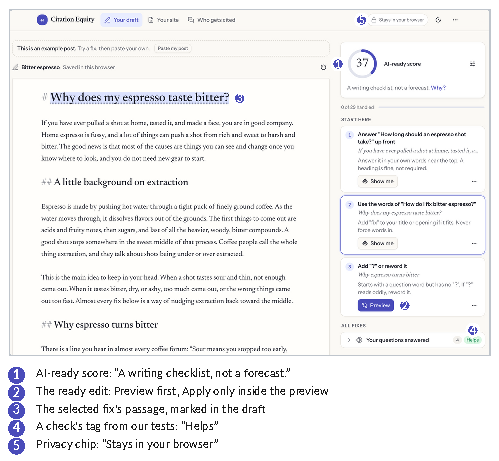
\includegraphics[width=\columnwidth]{figures/fig2_workspace.pdf}
  \Description{A screenshot of the workspace's draft view on the espresso example. Left: the draft as a paper-style page, with its title underlined because the selected tip is about it. Right: the AI-ready score of 37 with the line "A writing checklist, not a forecast", three Start-here fixes (two tips and one ready edit with a Preview button), and the first fix group with the tag "Helps". Top right: a "Stays in your browser" chip. Numbered callouts point to each.}
  % takeaway rewritten 2026-10-26: since CE 008e68e the draft view shows no grades; a fix group carries at most one chip,
  % "Helps" or "Not scored" (CE/apps/workspace/components/check-chip.tsx; CE/README.md line 21); grades live on /research.
  \caption{\figtakeaway{The deployed draft view (espresso example): the author applies one fix at a time; a tag marks the checks our tests found to help.}}
  \label{fig:workspace}
\end{figure}

% sections/evidence.tex: Section 3, what the tests of the advice found (one outcome metric: the rank-based citation score
% of the one-change-at-a-time tests, CE/experiments/RESULTS_E1.md, CE/experiments/RESULTS_E2.md, CE/experiments/RESULTS_E3.md).
% Draft 2, 2026-10-24: cut from about 1,430 to about 640 words to fit 4 pages (notes/CUTS.md).
% Clarity pass, 2026-10-26 (notes/CLARITY-PASS.md): prose cut from about 540 to about 360 words. The laptop bench (word share) and the
% sensitivity test (citation share) are one sentence each, as context; method detail is one sentence plus the Research
% page; results name checks, not experiment arms; numbers that Figure 4 shows were dropped from the text. The nine
% sources' citations moved to Section 2.1 (sec:checks).
%   CE     = ../citation-equity (tool repo, read only; numbers first checked at commit f38d34e, src pointers rechecked
%            at the feat head c908431 on 2026-10-26; public main b10887e has the same files except CE/docs/superpowers and CE/docs/research/*.json)
%   S-JSON = CE/experiments/results/sensitivity/sensitivity_{Qwen__Qwen3.5-9B, google__gemma-4-12B-it,
%            Qwen__Qwen3.8-27B, google__gemma-4-31B-it}.json
% Every number carries a "% src:" comment. Derived numbers cite data/sensitivity_derived.json (scripts/derive_sensitivity.py).
% "E1", "E2" and "E3" are named only in comments (and once in the E4 owner mark); the prose says "our first test" and
% "follow-up tests".

\section{What the tests found}\label{sec:evidence}\label{sec:findings}

% src: CE/samples/README.md lines 43 to 50 ("The first recording, and why it was superseded"; CE c908431): 4,096-token default window,
%      prompts about 3,500 tokens, 3 truncated calls; 13 of 128 answers without a valid [n]; no chance level reported
% src: p floor: CE/samples/README.md line 98 ("With 4 questions the smallest possible p is 0.125, so these runs can show a direction
%      at most.")
% src: CE/samples/README.md lines 81 and 87 to 98 (llama3.2:3b, 128 answers all valid; 5.3 to 6.5 of 8 sources cited;
%      word share 0.087 -> 0.137 and 0.086 -> 0.095; chance 0.125 inside every 95% interval; paired p 0.25 and 0.75,
%      smallest possible 0.125)
On the authors' laptop the bench shows a direction at most: every 95\% interval of the draft's word share included the 0.125 chance level, $p \geq 0.125$ with 4 questions, and a first recording, misread through truncated prompts, was withdrawn.
% src: CE/experiments/RESULTS_sensitivity.md and data/sensitivity_derived.json (unchanged from draft 2): 4 models x 256
%      valid answers, 8 questions x 8 seeds, 7 synthetic competitors, no retrieval; plan 3c86c02 before results 4d77fa0
%      (CE/experiments/PREREG_sensitivity.md, "Criteria (fixed before running)"); answer edit +0.007 to +0.034 vs bar
%      +0.10, detectable difference for the answer edit (mde_post_hoc of answer_first_minus_before) 0.019 to 0.047, below
%      the bar (data/sensitivity_derived.json "ranges"."mde_post_hoc_answer_first"); after draft +0.014 to +0.031;
%      drafts 14% and 22% longer (`wc -w` on CE/samples/*/{before,after}.md, rechecked 2026-10-26: 831 -> 946 and
%      1,041 -> 1,275); off-topic control <= 0.0031 (shown in Figure 1b)
A sensitivity test planned in advance, with four open models and synthetic competitors, measured \emph{citation share}: a one-sentence answer edit gained only $+0.007$ to $+0.034$ against a $+0.10$ target the harness could detect, and the full after drafts, 14\% and 22\% longer, gained $+0.014$ to $+0.031$ (Figure~\ref{fig:overview}b).

\paragraph{One change at a time.}
% src: CE/experiments/PREREG_E1.md (frozen r3 at 7859b07, before any page was edited; amendments 1-10 at its end) and
%      CE/experiments/RESULTS_E1.md (commit e258a1a; data/e1_results.json): 80 main queries (GEO-bench test split,
%      informational), 60 C-SEO Bench queries; editor Gemma-4-31B-it edits only the flagged spans, validators reject edits
%      that add facts or miss the check; reference = a same-length paraphrase of the same spans; 4 sources per prompt, slot
%      rotated; judges Gemma-4-12B-it and Qwen3.8-27B, 8 seeds; score (5 - r)/4 with r = 5 if uncited
%      (CE/experiments/PREREG_E1.md line 119); 17,823 of 17,824 answers valid (CE/experiments/e1/out/score_summary.json);
%      plans for the follow-ups: CE/experiments/PLAN_E2.md line 3 and CE/experiments/PLAN_E3.md line 3
% src: Research page https://shehral.github.io/citation-equity/research/ (HTTP 200 on 2026-10-26; reports E1 to E3 with
%      Holm-adjusted results), listed with the code and data in the intro footnote (fn:links)
Our first test applies one check's suggestion alone to real pages (80 informational GEO-bench queries~\cite{aggarwal2024geo}, replicated on 60 from C-SEO Bench~\cite{puerto2025cseo}): an open model edits only the spans the check flags, and each edit is compared with a same-length paraphrase of those spans; two open judges see the page among 4 sources, and its \emph{citation score} is $(5-r)/4$ when it is the $r$-th source cited, else 0 (plans fixed in advance, code and data: footnote~\ref{fn:links}).

% src: CE/experiments/RESULTS_E1.md main primary contrasts: arm 9 (target questions answered, done as a section headed by
%      the question) +0.027 [+0.010, +0.043] Holm 0.006 n 54, replication +0.036 n 52; arm 12 (query words in title and
%      lead = the reader's-words check) +0.035 [+0.008, +0.066] Holm 0.037 n 33; confound-adjusted intercepts include 0
%      (arm 9 [-0.075, +0.018], arm 12 [-0.083, +0.018], ALL-original [-0.012, +0.096]); data/e1_results.json "main",
%      "replication"; all fixes (ALL +0.049 n 78, +0.071 vs P_ALL n 53, replication +0.044) are shown in Figure 4 only
Of single changes, only the two that add the reader's own words near the top clearly raised the score (Figure~\ref{fig:e1}): \emph{target questions answered}, done as a section headed by the question ($+0.027$, 95\% CI $[+0.010, +0.043]$, Holm $p = 0.006$; replication $+0.036$), and \emph{your reader's words up top}, the question's missing words in title and lead ($+0.035$); for both, the effect left after regressing out length and question-word changes includes zero.
% src: CE/experiments/RESULTS_E2.md, E2a planned tests (d = arm 9 minus 9W or 9P; data/e1_results.json "e2"."e2a"):
%      9 vs 9W main +0.003 [-0.009, +0.016] n 54, replication -0.001 [-0.014, +0.012] n 52, both "no effect larger
%      than delta"; 9 vs 9P replication +0.048 [+0.027, +0.071] Holm p < 0.001 "helps", main +0.017 [+0.001, +0.033]
%      Holm 0.089 "inconclusive" (both shown in Figure 4 only; the text no longer states them); reported without a verdict: 9W vs original +0.023 (main) and
%      +0.037 (replication)
Follow-up tests, each planned before its answers, place the gain in the words, not the form: the question heading did no better than the same text set as plain ($+0.003$; replication $-0.001$) while the plain-text question scored higher than the untouched page ($+0.023$; $+0.037$).
% src: CE/experiments/RESULTS_E2.md, E2b (editor Qwen3.8-27B; judges Gemma-4-12B and Qwen3.5-9B; data/e1_results.json
%      "e2"."e2b"): 12 vs P12 +0.029 [+0.003, +0.061] n 29; ALL vs P_ALL +0.069 [+0.038, +0.104] n 44; both keep E1's sign
With another editor and other judges, the reader's-words gain kept its sign ($+0.029$, $n = 29$), as did all fixes together ($+0.069$, $n = 44$).
% src: CE/experiments/RESULTS_E3.md "Pooled result" (data/e1_results.json "e3"; 260 queries, 180 new): arm 2 -0.016
%      n 57, arm 7 -0.010 n 49, arm 8 +0.012 n 66 "no effect larger than delta"; arm 6 +0.026 [+0.001, +0.053] n 62
%      Holm 0.179 "inconclusive"; arms 4, 5, 10 n 11, 11, 24 (all shown in Figure 4); "Where the queries come from"
%      (E1's queries gained at most 4 pairs from the extra attempt; the editor runs at temperature 0,
%      CE/experiments/PREREG_E1.md line 85); lists: E1 arm 3 -0.007 n 33 "no effect larger than delta" (RESULTS_E1.md)
A second follow-up added 180 queries for the checks with too few pages: over 260, question headings, cited sources and direct answer first showed no effect larger than 0.03 and attributed quotes were inconclusive; tables, statistics and comparisons still had too few.
% The owner approved this tool update (task brief, 2026-10-24). The rule's outcome (four unscored notes, the new reader's-words
% check) is stated once, in Section 2.1 (sec:checks); the sentence that repeated it here was cut (notes/CUTS.md 68).
% src for that outcome: CE commits 27201da (reader-words check), 8219c90 (measured fixes first) and 00d65b7 (E3's pooled
%      results; question headings, cited sources, direct answer first unscored), merged at 4831ff9; CE/docs/evidence.md line 34 (CE c908431)
% Reserved space (clarity pass 2026-10-26): about 4 lines for the Gemini judge check of the three key comparisons; the
% build was checked with 4 lines of filler here (notes/CLARITY-PASS.md).
% E4 (a Gemini judge check) was stopped before analysis on 2026-10-26 (free-tier quota); see CE/experiments/PLAN_E4.md. Nothing reported.

% ---------------------------------------------------------------------------------------------------------------
\begin{figure}[t]
  \centering
  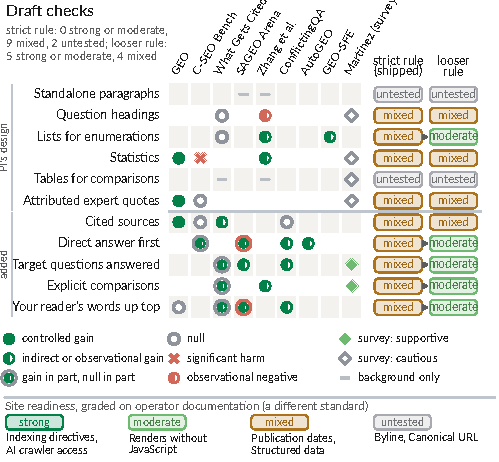
\includegraphics[width=\columnwidth]{figures/fig3_evidence.pdf}
  \Description{A matrix with the eleven draft checks as rows and the nine sources as columns. Each cell marks a controlled gain, an indirect or observational gain, a gain in part with a null in part, a null, a significant harm, an observational negative, survey support or caution, or background only. Two chip columns give each check's grade under the strict shipped rule (9 mixed, 2 untested) and under a looser rule (5 moderate, 4 mixed, 2 untested). A strip below grades the seven site-readiness items.}
  % src (caption): CE/docs/evidence.md line 34; data/evidence_grades_loose.json tally (strict 0/0/9/2; loose 0/5/4/2);
  %      readiness_tally 2 strong, 1 moderate, 2 mixed, 2 untested; single-rater coding (data/README.md)
  % cite order in the caption = the columns, left to right (moved from Section 3's "The grades" in the clarity pass)
  % columns, left to right, follow scripts/figdata.py STUDIES (CE/docs/evidence.md table rows at lines 80 to 88); rows follow the
  %      engine registry (eleven checks; reader's words last, coded from CE/docs/evidence.md lines 255 to 258); cell lines in
  %      data/evidence_matrix.csv remapped to CE c908431 on 2026-10-26 (+2 after line 37, identical text)
  \caption{\figtakeaway{Every tested draft check has a null or negative result somewhere, but ``mixed'' spans positive-in-every-model to harmful, and a looser rule, defined post hoc, moves five to moderate.}
    Columns: \cite{aggarwal2024geo}, \cite{puerto2025cseo}, \cite{vishwakarma2026cited}, \cite{kim2026sageo}, \cite{zhang2026absorption}, \cite{wan2024conflictingqa}, \cite{wu2026autogeo}, \cite{yu2026geosfe}, \cite{martinez2026survey}. One rater.}
  \label{fig:evidence}
\end{figure}

\begin{figure}[t]
  \centering
  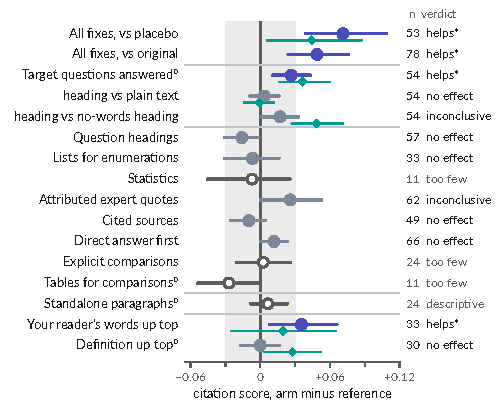
\includegraphics[width=\columnwidth]{figures/fig4_e1.pdf}
  \Description{A forest plot over real web pages. Each row is one check's suggestion applied alone, or all fixes together, with the mean difference in citation score from its reference and a 95 percent interval, a shaded band from minus 0.03 to plus 0.03, and small teal diamonds for the 60-query replication. All fixes together, target questions answered and your reader's words up top sit to the right of the band. Two rows under target questions answered compare its question heading with the same text as plain text (near zero) and with a heading without the question's words (positive, clearly so in the replication). Question headings, lists, cited sources and direct answer first sit inside the band; attributed expert quotes is inconclusive; statistics, explicit comparisons and tables for comparisons have open circles with too few pages.}
  % src (caption): data/e1_results.json ("main", "replication", "e2", "e3"); scripts/fig_e1.py (row names = Figure 3's check names)
  % Clarity pass: "260 queries for question headings and statistics to tables, 80 for the rest" dropped (Section 3 says which
  % checks the 260-query follow-up covers; notes/CUTS.md 79).
  \caption{\figtakeaway{Of single changes, only the two adding the reader's words up top clearly raised citation; the heading form, sources and answer-first showed no effect larger than 0.03; quotes were inconclusive.}
    Difference from a same-length paraphrase or the original ($^{\circ}$), 95\% intervals; filled: 30+ pages; band: $\pm 0.03$; teal: replication; helps$^{*}$: possibly via question-word overlap.}
  \label{fig:e1}
\end{figure}

\begin{figure}[t]
  \centering
  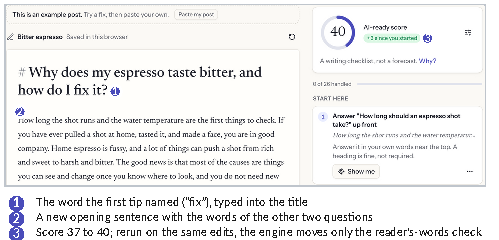
\includegraphics[width=\columnwidth]{figures/fig5_reader_words.pdf}
  \Description{A screenshot of the deployed draft view on the espresso example after two edits. Left: the title now reads "Why does my espresso taste bitter, and how do I fix it?" and the first paragraph opens with "How long the shot runs and the water temperature are the first things to check." Right: the AI-ready score of 40 with a green chip "+3 since you started", the line "A writing checklist, not a forecast", and the first Start-here fix. Numbered callouts mark the title words, the opening sentence and the chip.}
  % src (caption): data/fig5_callouts.json (scripts/capture_reader_words.mjs, live site 2026-10-26): score_before "AI-ready
  %      score: 37 out of 100", score_after "... 40 out of 100", chip "+3 since you started", tips read before each edit
  %      (first: Add "fix"; second: Add "long"; none left after the opening sentence); "engine" block: the tool repo engine
  %      (CE c908431) on CE/samples/espresso-bitterness/before.md and the same two edits, the four sample questions as
  %      questions and reader's questions: Standard 37 -> 40, only reader-words changed (0.667 -> 1.000)
  \caption{\figtakeaway{Following the reader's-words tips raises the score: the tool now scores what helped.}}
  \label{fig:readerwords}
\end{figure}

% sections/related.tex: related work. Draft 2, 2026-10-24: cut from about 275 to about 150 words (notes/CUTS.md).
% Keys: aggarwal2024geo (R1), puerto2025cseo (R2), vishwakarma2026cited (R4), kim2026sageo (R3), wu2026autogeo (R10),
%   bajemon2026scoring (R39, preprint, vendor-linked), aiseoaudit (CE/docs/research/2026-10-23-oss-sweep.json, local feat branch only),
%   geoscore (R238). Rnnn = ids in our internal landscape corpus (not public).

\section{Related work}\label{sec:related}

% src: CE/NOTICE lines 10 to 25 (CE/packages/bench/src/prompt.ts and CE/packages/bench/src/metrics.ts adapted from GEO-optim/GEO,
%      Apache-2.0); corpus R3 (visibility per stage);
%      corpus R10 (automatic rewriter); corpus R39 summary and verifier_note; CE/docs/research/2026-10-23-oss-sweep.json lines 14 and 201 (aiseo-audit FACTOR_REGISTRY with
%      evidence tiers; lists, tables and answer capsules tagged 'diagnostic'); CE/NOTICE lines 29 to 39 (code adapted from aiseo-audit 2.1.2,
%      commit 6c888aa);
%      corpus R238 (geo-score keeps citation tracking out of the score)
The bench reuses GEO's prompt and word share~\cite{aggarwal2024geo} and the counterfactual style of C-SEO Bench and What Gets Cited, which edit one page and hold the rest fixed~\cite{puerto2025cseo,vishwakarma2026cited}.
Bajemon and Rochet validate a content score against engines through falsification gates~\cite{bajemon2026scoring} (a vendor-linked preprint); we run no such validation and do not claim our score predicts citation.
Among open tools, aiseo-audit keeps an evidence tier for every factor and already demotes lists and tables to unscored diagnostics~\cite{aiseoaudit}, and Citation Equity adapts code from it.
% src: none of the 341 sources in our internal landscape corpus (not public) is a
%      user study of a GEO tool (its user studies, R53 and R88 to R121, study answer engines or AI writing tools); verify-claims B8

% sections/demo.tex: Section 5, the demonstration at the venue (required by the WWW 2027 demo call).
% Draft 2, 2026-10-24: cut from about 275 to about 190 words (notes/CUTS.md).
% CE = ../citation-equity (the tool repo, read only). Every number carries a "% src:" comment.

\section{Demonstration at the venue}\label{sec:demo}

% src: CE/samples/README.md line 82 (Apple M4 Pro, 24 GB, Ollama 0.40.9); CE/README.md lines 40 to 47 (Ollama setup), CE c908431
One laptop serves the static build and runs Ollama (\texttt{llama3.2:3b}), so the core demonstration needs no venue network.
A second screen shows the hosted demo, and a poster carries Figures~\ref{fig:overview} and~\ref{fig:e1}.

% src (Station 1, CE c908431): Start here on the example = the reader-question advice, the reader's-words advice and the
%      example's only ready edit, the heading "?" (an unscored note, kept by "Start here always keeps one ready edit":
%      CE/packages/engine/src/rank.ts lines 69 to 95, CE commit 5e7ac43; CE/README.md line 20). Rechecked 2026-10-26 with the
%      engine source (analyze with the four pack questions as questions and authorQuestions, rankFixes, startHereFixes):
%      score 37; the "?" edit leaves 37; working the questions' words into the opening raises it (reader's words weight 0.5).
%      Figure 2 shows the same three fixes.
% src: CE/samples/README.md lines 81 and 83 (64 answers = 2 drafts x 4 questions x 8 runs; espresso 18:37 to 18:52 PDT)
\emph{Station 1, the 90-second loop.} The visitor loads the espresso example, follows the reader's-words advice and watches the score change (Figure~\ref{fig:readerwords}), applies a ready edit through Preview (a heading's question mark, an unscored note, so the score holds), opens the studies behind one mixed check and the recorded citation test beside its chance line.
A live run (64 answers, 15 minutes) starts each session and fills in while visitors watch.
\emph{Station 2, bring your own text (offline).} Visitors paste their own paragraph and see checks, suggestions and grades; the text never leaves the laptop.
% src: CE/README.md line 59 (ce site); CE/docs/evidence.md line 262 (five items in the browser, two need a fetch: ce site), CE c908431
\emph{Station 3, can engines reach your site? (online).} The command-line \texttt{ce site} runs the seven readiness items on the visitor's URL over a phone hotspot; offline, pasted HTML runs five of them in the browser.

% sections/conclusion.tex: Ethics and use of data as its own section (required by the WWW 2027 demo call, notes/VENUE.md), limitations, future work,
% acknowledgments and the AI-use statement placeholder.
% Draft 2, 2026-10-24: cut from about 375 to about 210 words (notes/CUTS.md). CE = ../citation-equity (read only).

\section{Ethics and use of data}\label{sec:ethics}

% src: CE/README.md line 68 ("The web app has no server"); CE/docs/cli.md line 89 ("Drafts stay on your disk unless you point
%      `ce bench` at a hosted server"), CE c908431
% src: CE/samples/README.md lines 27 to 31 (packs and pages synthetic, people fictional); CE/NOTICE lines 133 to 145 (C-SEO Bench
%      "Data used at run time (not redistributed)"); CE/docs/cli.md line 22 (`ce pack from-urls` "respects robots.txt")
% src: CE/docs/evidence.md lines 456 and 492 (FTC review rule and Endorsement Guides; line numbers at CE c908431)
No human participants took part and no user data was collected.
Sample drafts and competitor pages are invented; C-SEO Bench is downloaded at run time, never redistributed; building competitor pages from URLs respects robots.txt.
% src: CE/README.md line 3 ("it suggests, you decide"); CE/docs/architecture.md line 84 (Rewrite with local AI only after a
%      click) and CE/apps/workspace/components/draft/draft-view.tsx lines 683 to 686 ("Nothing is applied here.")
On dual use, it generates no page text on its own, asks for real and checkable material, and states the FTC's endorsement rules; the bench could test a manipulative edit, but the tool offers none.
% src: CE/experiments/PREREG_E1.md line 18 (GEO-bench source URLs: research use only, never redistributed; only aggregates
%      and hashes committed). Owner item (notes/STATUS.md): Prof. Akram confirms this research use before submission.
% As PREREG_E1.md line 18 planned: no page text, and nothing built from it, is redistributed (2026-10-29).
The tests use the public pages GEO-bench lists~\cite{aggarwal2024geo}; their text, and everything built from it, is not redistributed, only URLs, hashes and results.
A future user study will go through IRB review.

% src: CE/experiments/PREREG_sensitivity.md lines 11 to 20; CE/samples/README.md lines 9 to 12, 27 and 55 ("Write in English");
%      Martinez Table 5
% src: 320 queries = 260 GEO-bench (E3 pooled, CE/experiments/RESULTS_E3.md) + 60 C-SEO Bench (CE/experiments/RESULTS_E1.md);
%      Gemma-4-31B-it edits all but E2b's (Qwen3.8-27B, 80 queries, CE/experiments/RESULTS_E2.md)
% src: CE/experiments/PREREG_E1.md line 114 (the byte-identity check against --export-prompts is planned for E1 only; the check
%      is CE/experiments/e1/check_prompt_twin.ts, in the freeze manifest CE/experiments/e1/freeze/MANIFEST.md line 39; no
%      recorded run of it is in the tool repo, so this sentence stays until the owner runs it)
% src: smoke test CE/experiments/results/smoke_google__gemma-4-12B-it.json (commit 20e2b3f, 20:09 PDT, before the
%      pre-registration 3c86c02): planted page cited in 8/8 valid answers, mean share 0.9688; one model, outside the design
\section{Limitations and future work}\label{sec:conclusion}
Every measurement uses open models over fixed sources, not live engines, which differ and drift~\cite{martinez2026survey}; the sensitivity test covers two synthetic topics and 8 questions, the one-change tests 320 English queries, nearly all edited by one model family, with no positive control in the sensitivity design.
% Owner item (notes/STATUS.md): run the 10-prompt --export-prompts byte comparison and drop this sentence, or keep it.
The harness prompt has not been byte-checked against the bench's.
Next are a comparison with live engines and a study with writers.

\begin{acks}
This work was done in Northeastern University's SPARK research program in San Jose; the experiments ran on Northeastern Research Computing's Explorer cluster.

% AI-use statement: drafted at the owner's request on 2026-10-24, kept broad at his request. WWW 2027 CFP: LLMs cannot be
% authors; authors are solely responsible for the text. ACM Policy on Authorship: disclose generative-AI use (acknowledgments).
\emph{Use of generative AI.} We used Claude (Anthropic) as an assistant for software development, experiment and analysis code, and writing and editing. The authors designed the study, checked the results and take full responsibility for the paper.
\end{acks}


\bibliographystyle{ACM-Reference-Format}
\bibliography{references}

\end{document}
